% generated by src/build_paper.py from reports/walkthrough/screens/capture_log.json
\subsection*{Multi-Agent Pipeline}
\begin{figure}[H]\centering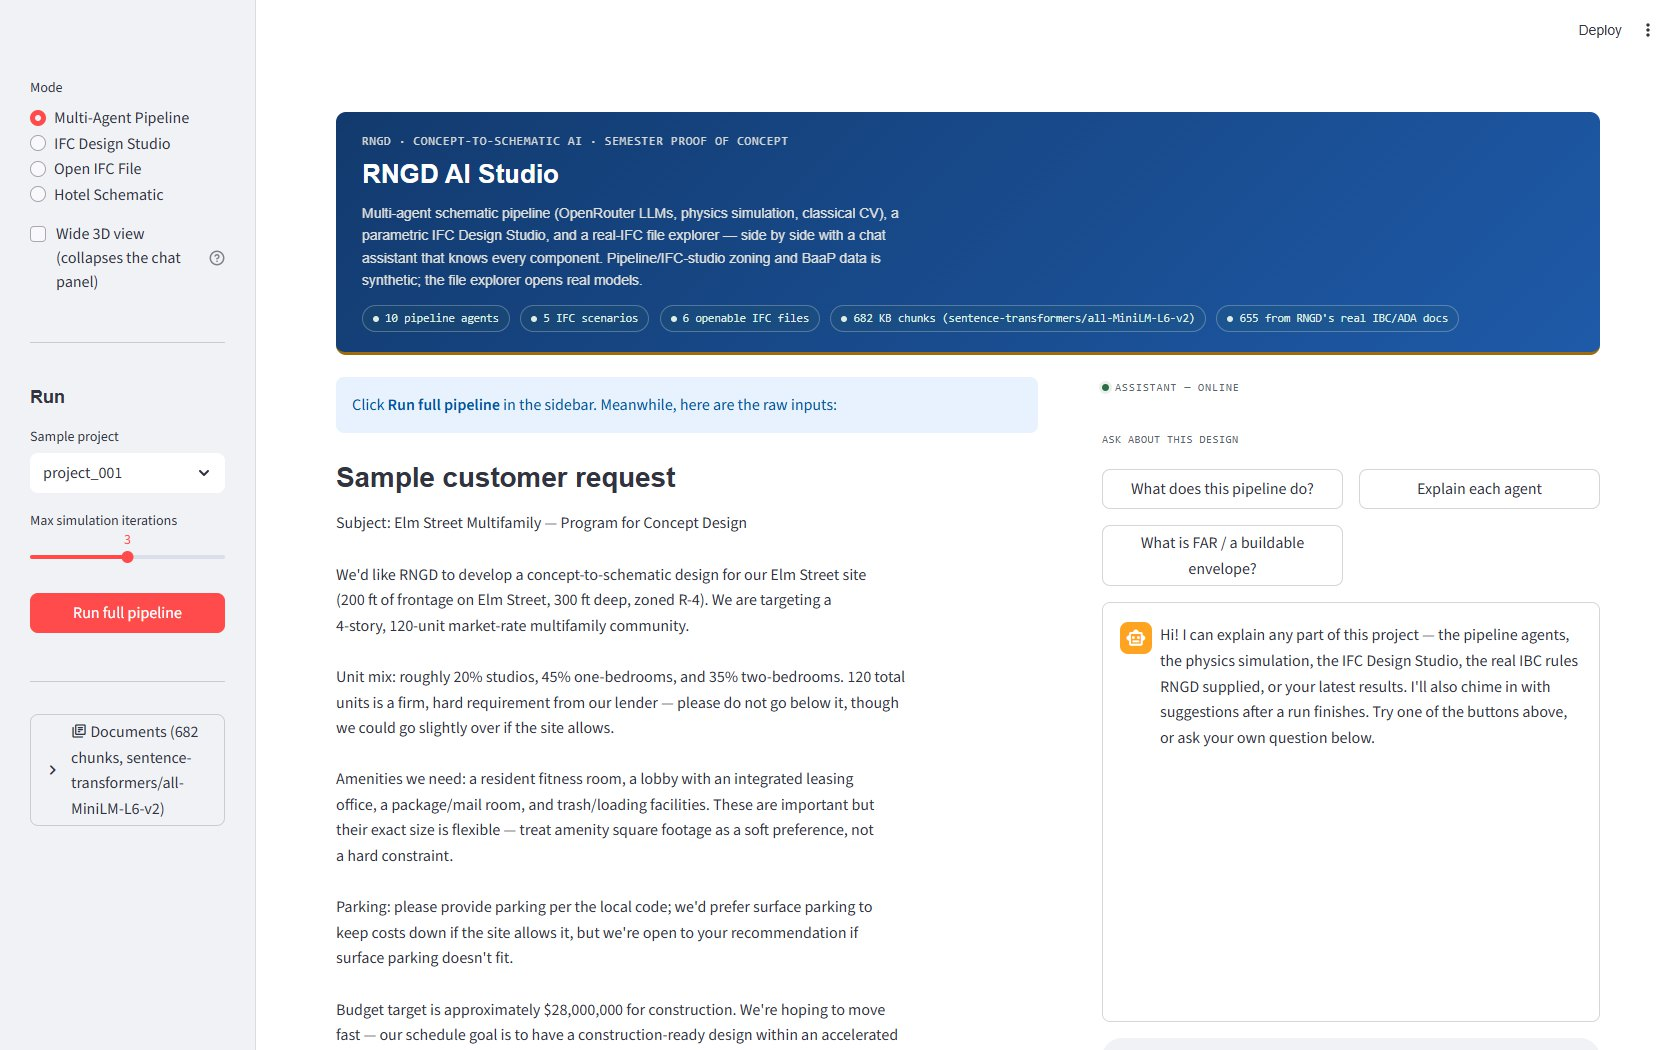
\includegraphics[width=0.92\linewidth,height=0.4\textheight,keepaspectratio]{figures/snap_01_pipeline_inputs}\caption*{\textbf{Screen 01.} Multi-Agent Pipeline before a run: the sample customer request and site sketch that feed the agents; the assistant panel on the right.}\end{figure}
\begin{figure}[H]\centering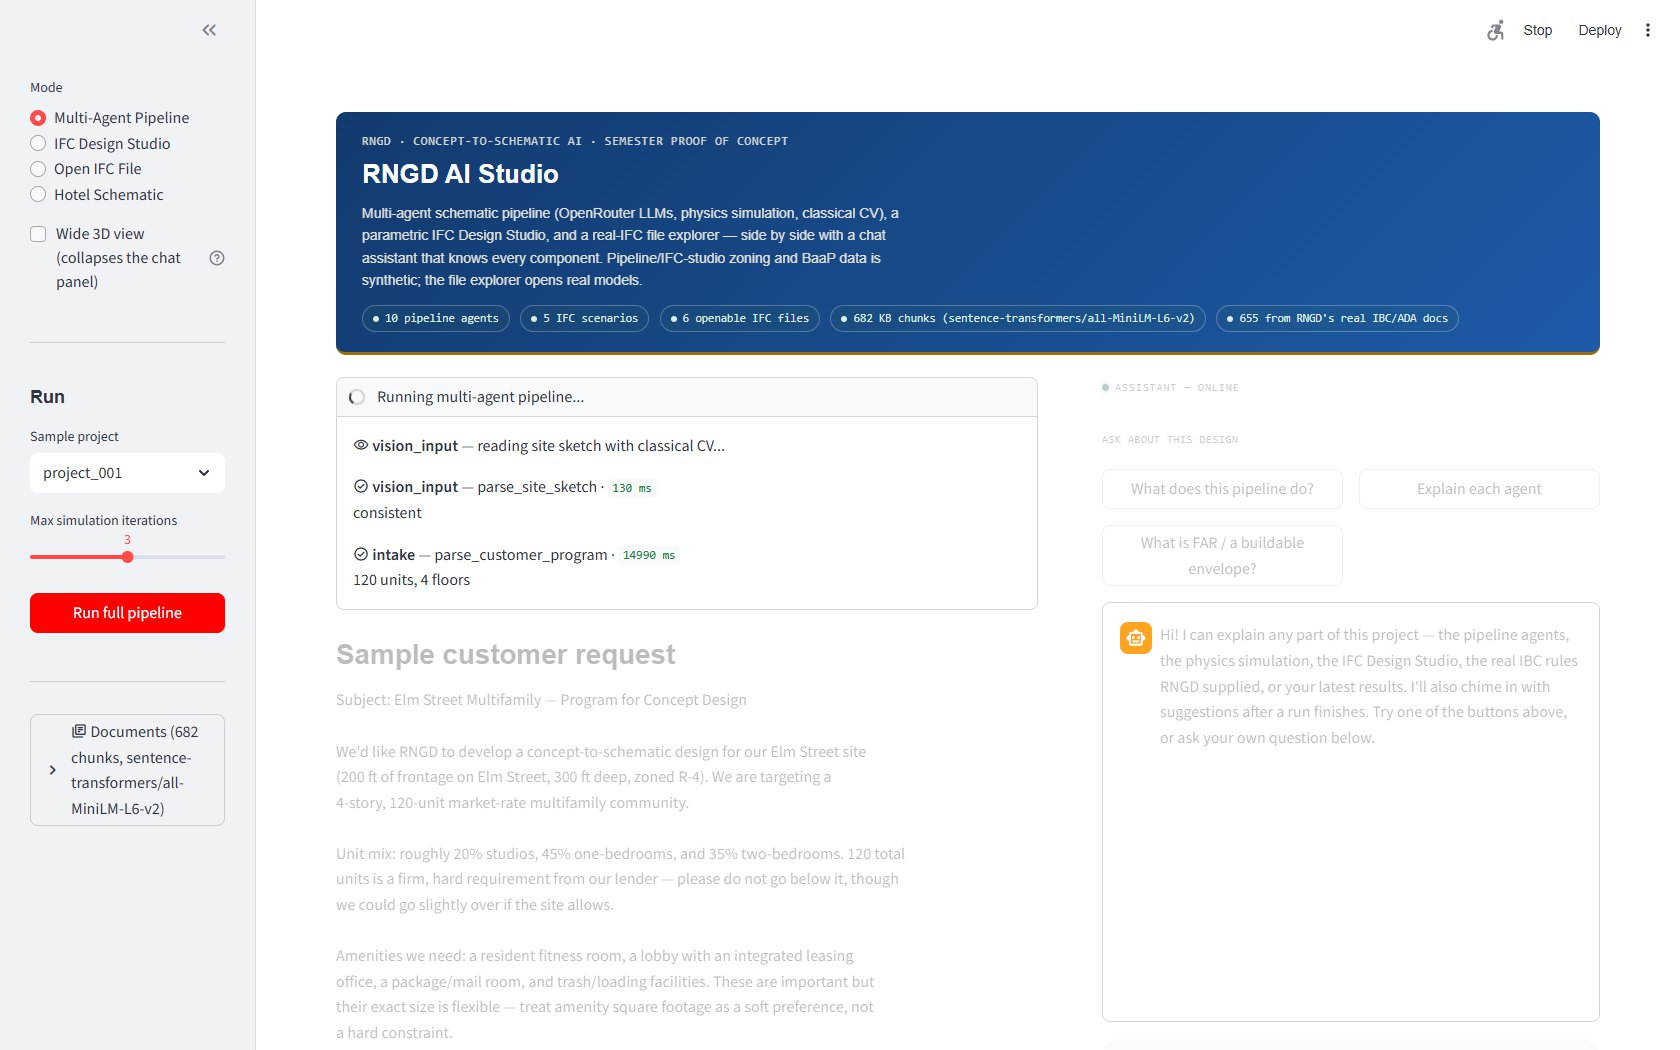
\includegraphics[width=0.92\linewidth,height=0.4\textheight,keepaspectratio]{figures/snap_02_pipeline_running}\caption*{\textbf{Screen 02.} The pipeline running live: each agent reports its step as it finishes.}\end{figure}
\begin{figure}[H]\centering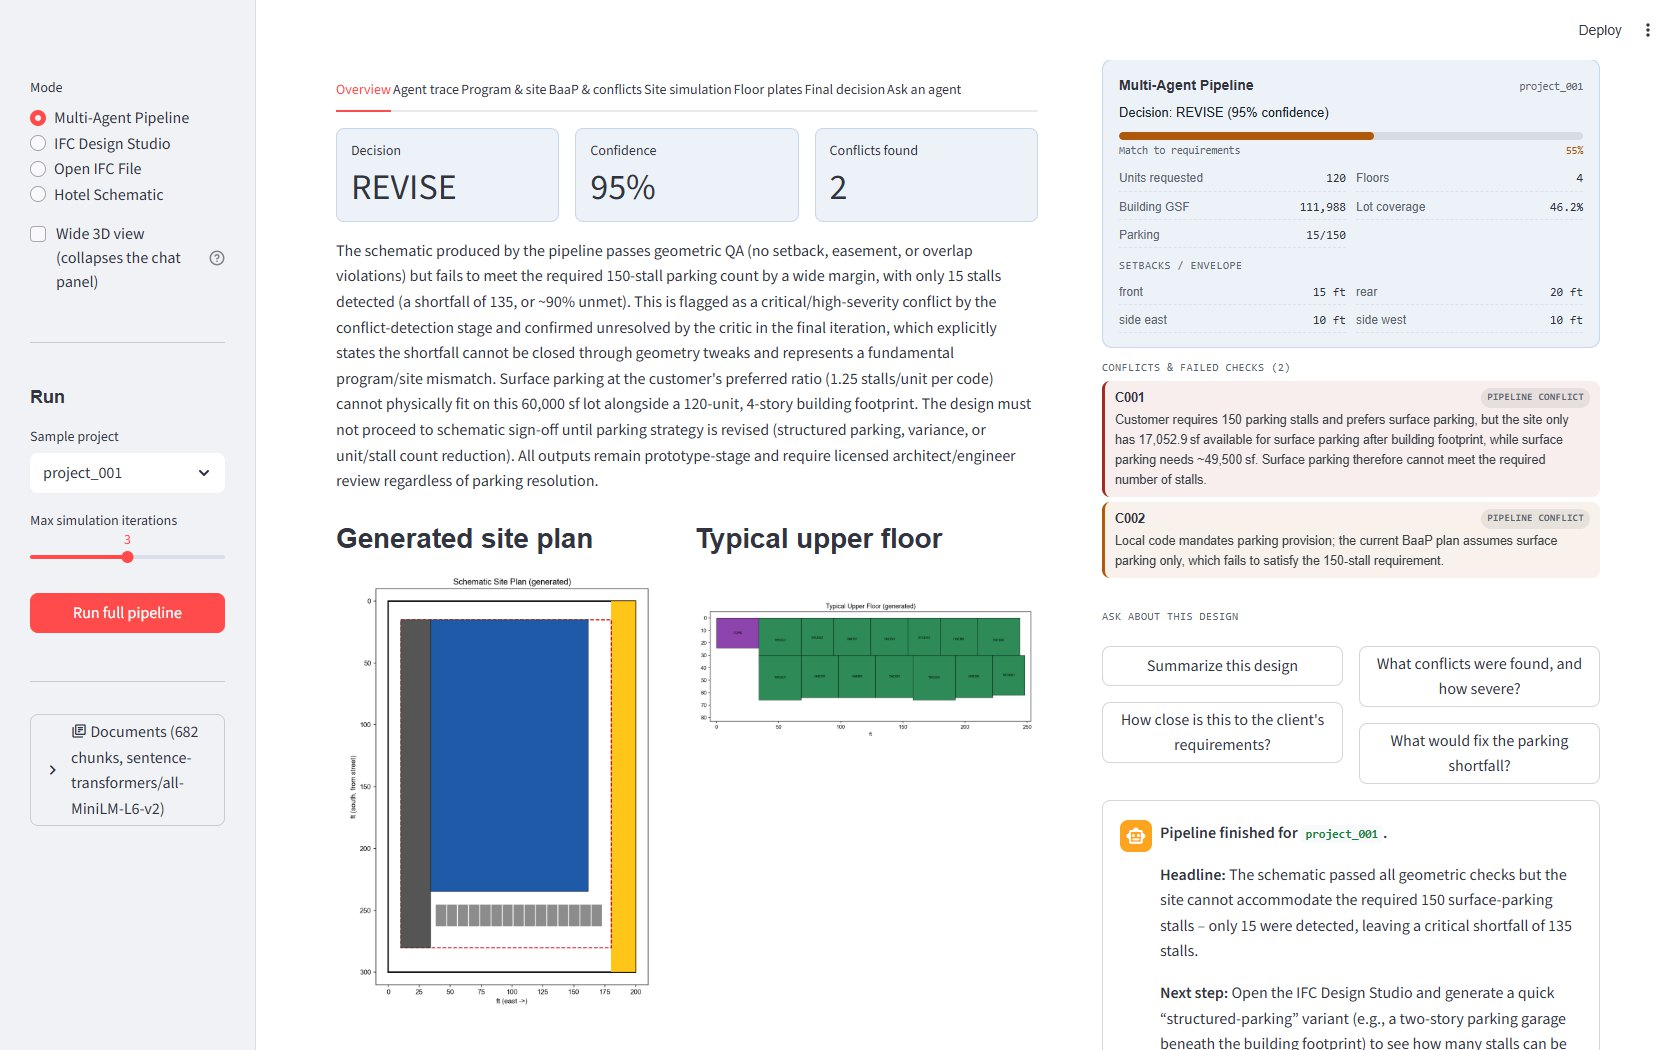
\includegraphics[width=0.92\linewidth,height=0.4\textheight,keepaspectratio]{figures/snap_03_pipeline_overview}\caption*{\textbf{Screen 03.} Pipeline result overview: the arbiter's decision, confidence and conflict count.}\end{figure}
\begin{figure}[H]\centering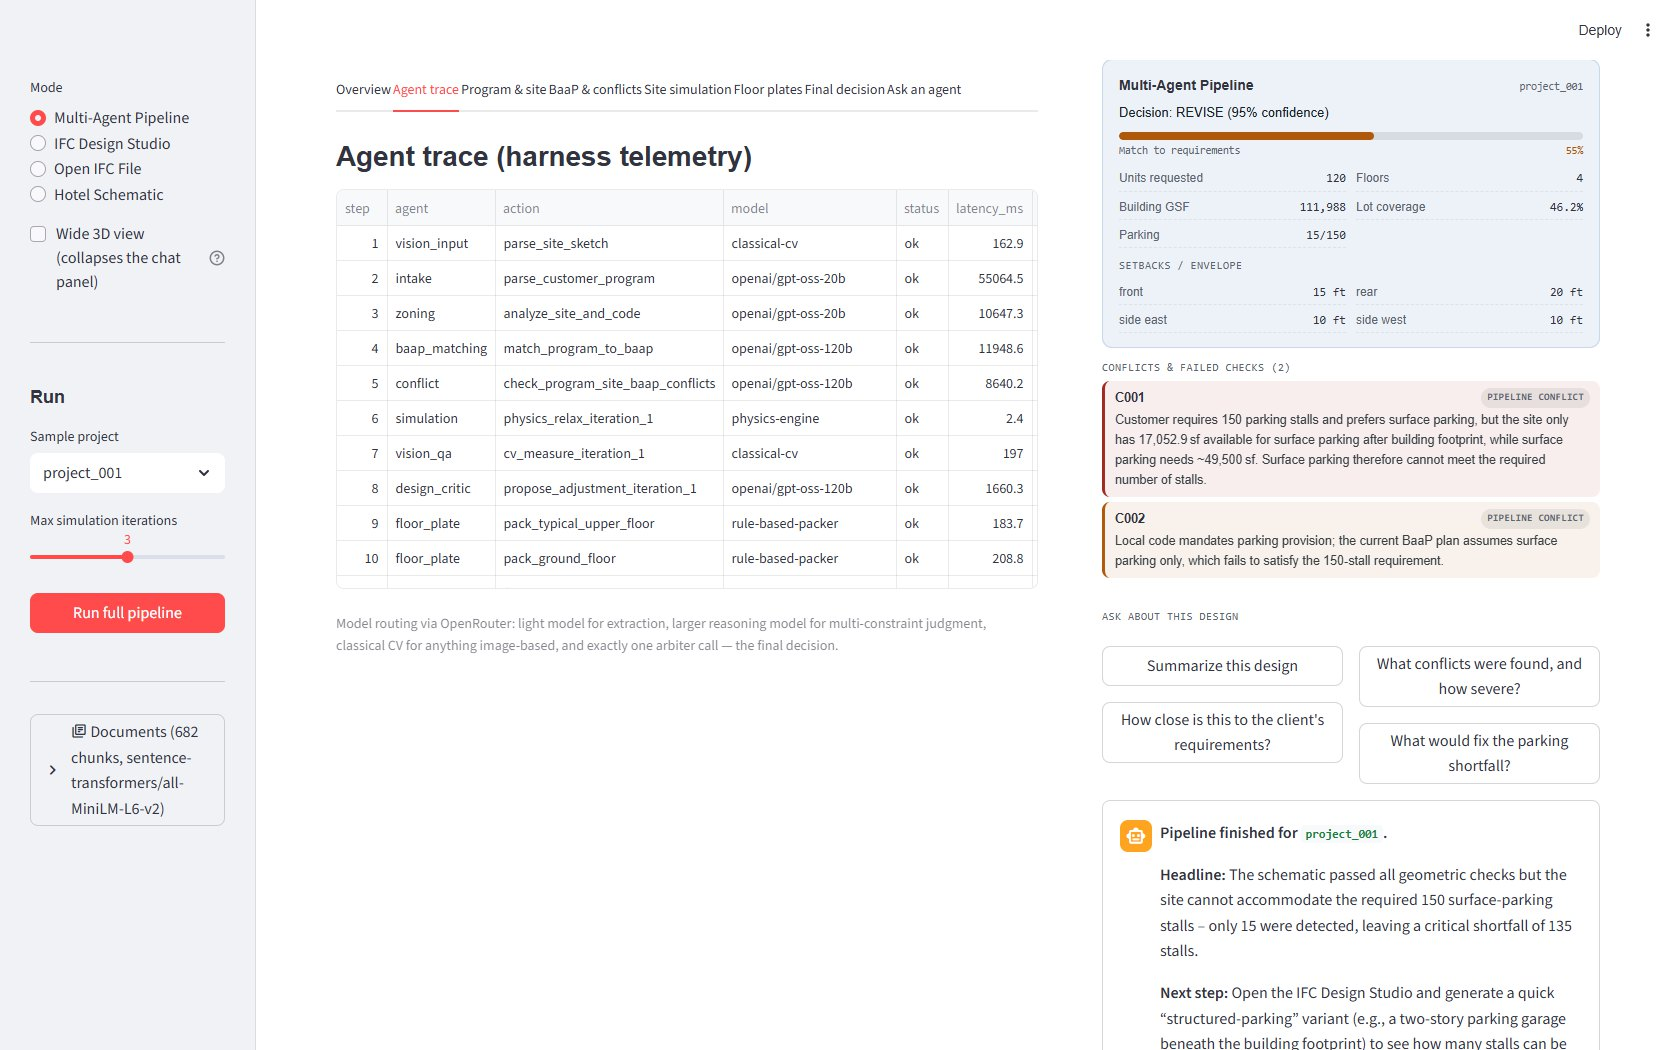
\includegraphics[width=0.92\linewidth,height=0.4\textheight,keepaspectratio]{figures/snap_04_pipeline_agent_trace}\caption*{\textbf{Screen 04.} Agent trace: every agent step with model, status and latency.}\end{figure}
\begin{figure}[H]\centering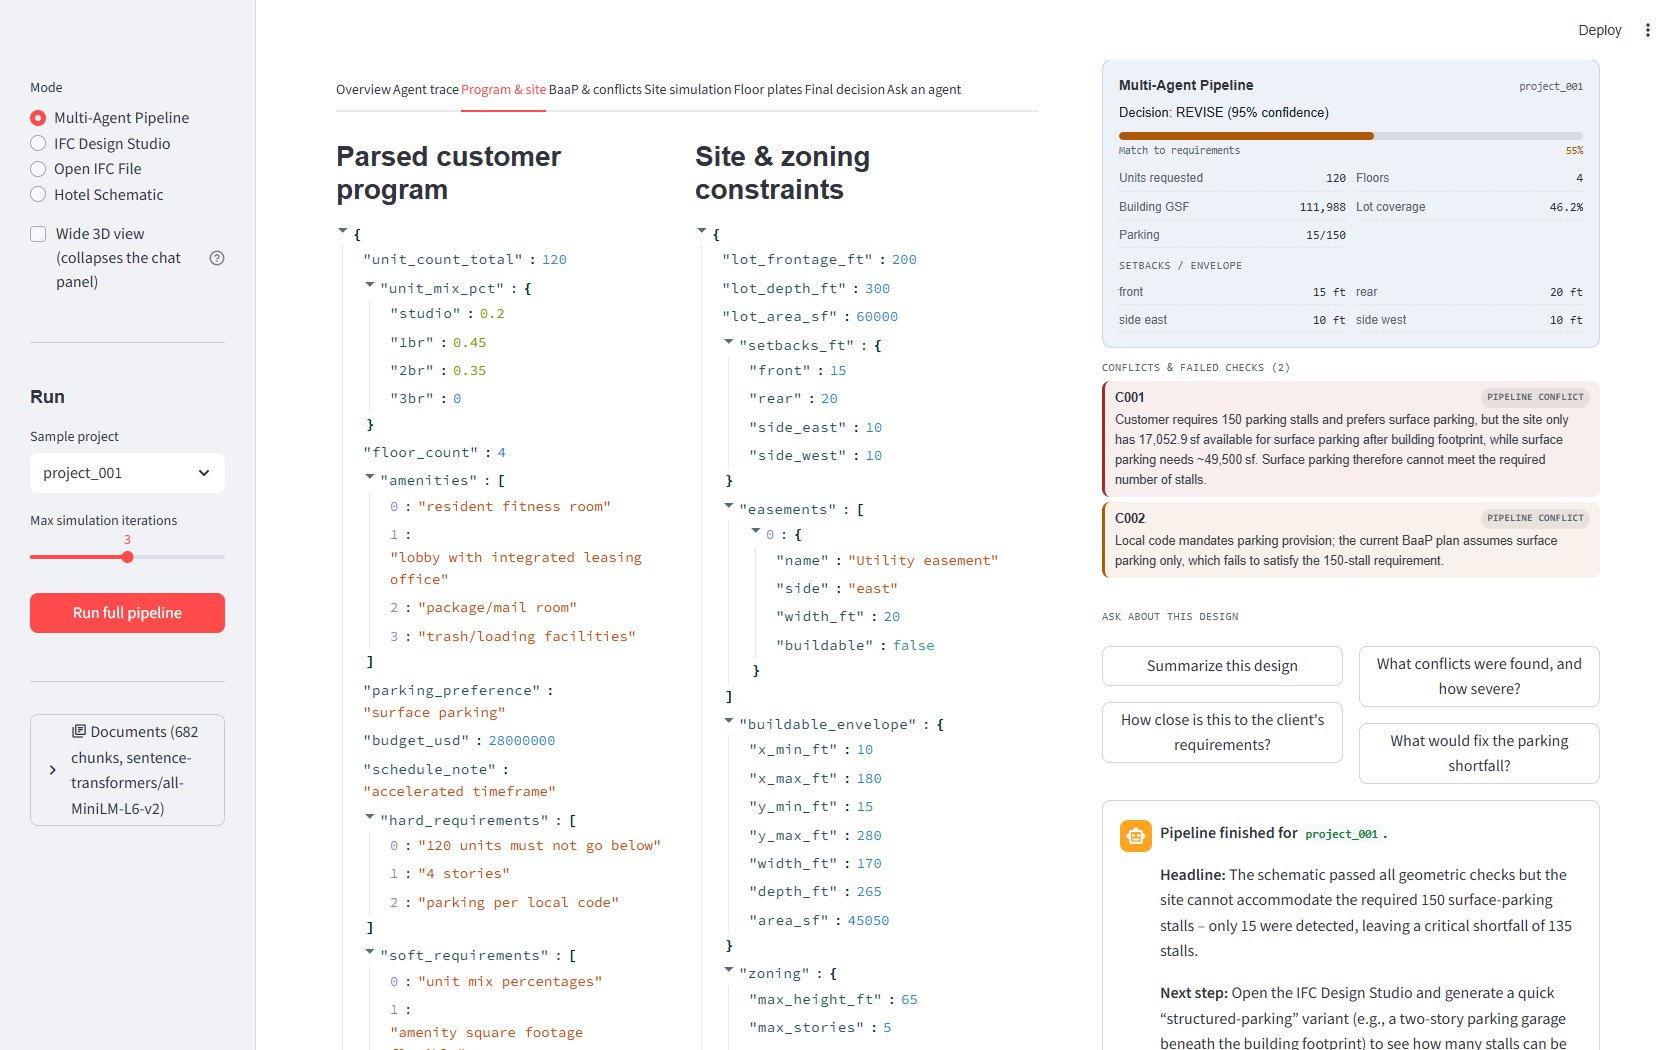
\includegraphics[width=0.92\linewidth,height=0.4\textheight,keepaspectratio]{figures/snap_05_pipeline_program_site}\caption*{\textbf{Screen 05.} Program parsed from the request and the computed site constraints.}\end{figure}
\begin{figure}[H]\centering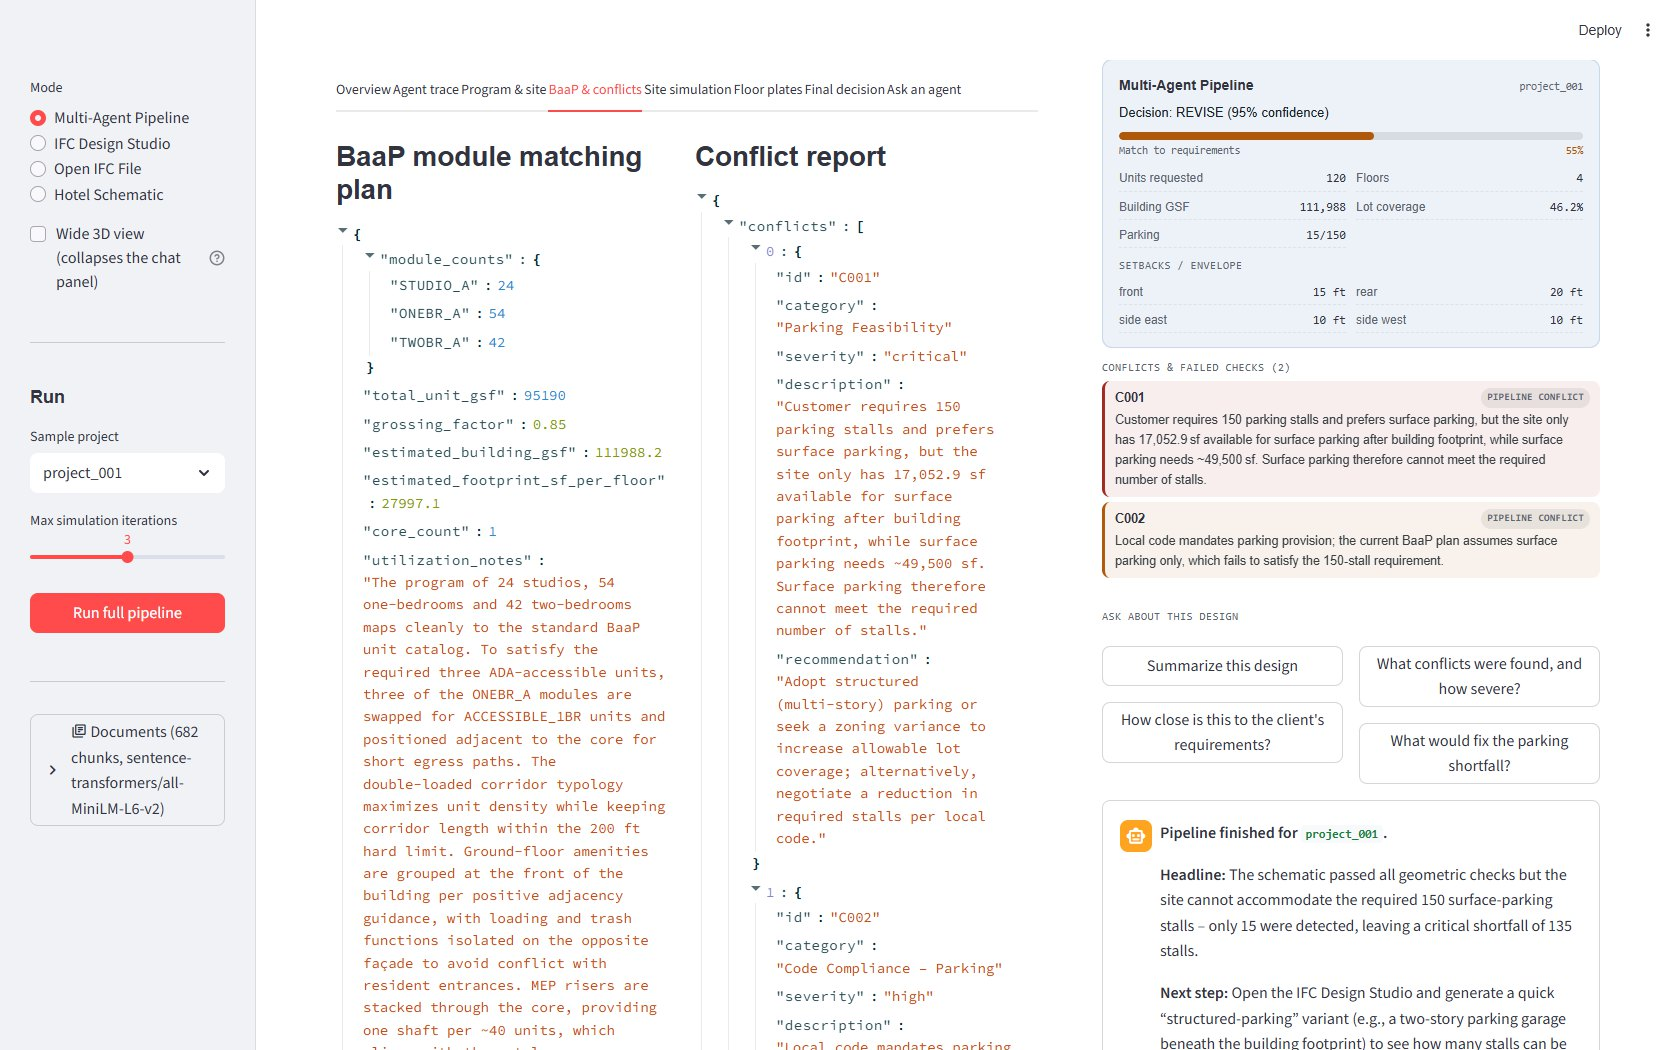
\includegraphics[width=0.92\linewidth,height=0.4\textheight,keepaspectratio]{figures/snap_06_pipeline_baap_conflicts}\caption*{\textbf{Screen 06.} BaaP module counts and the conflicts the Conflict Agent found.}\end{figure}
\begin{figure}[H]\centering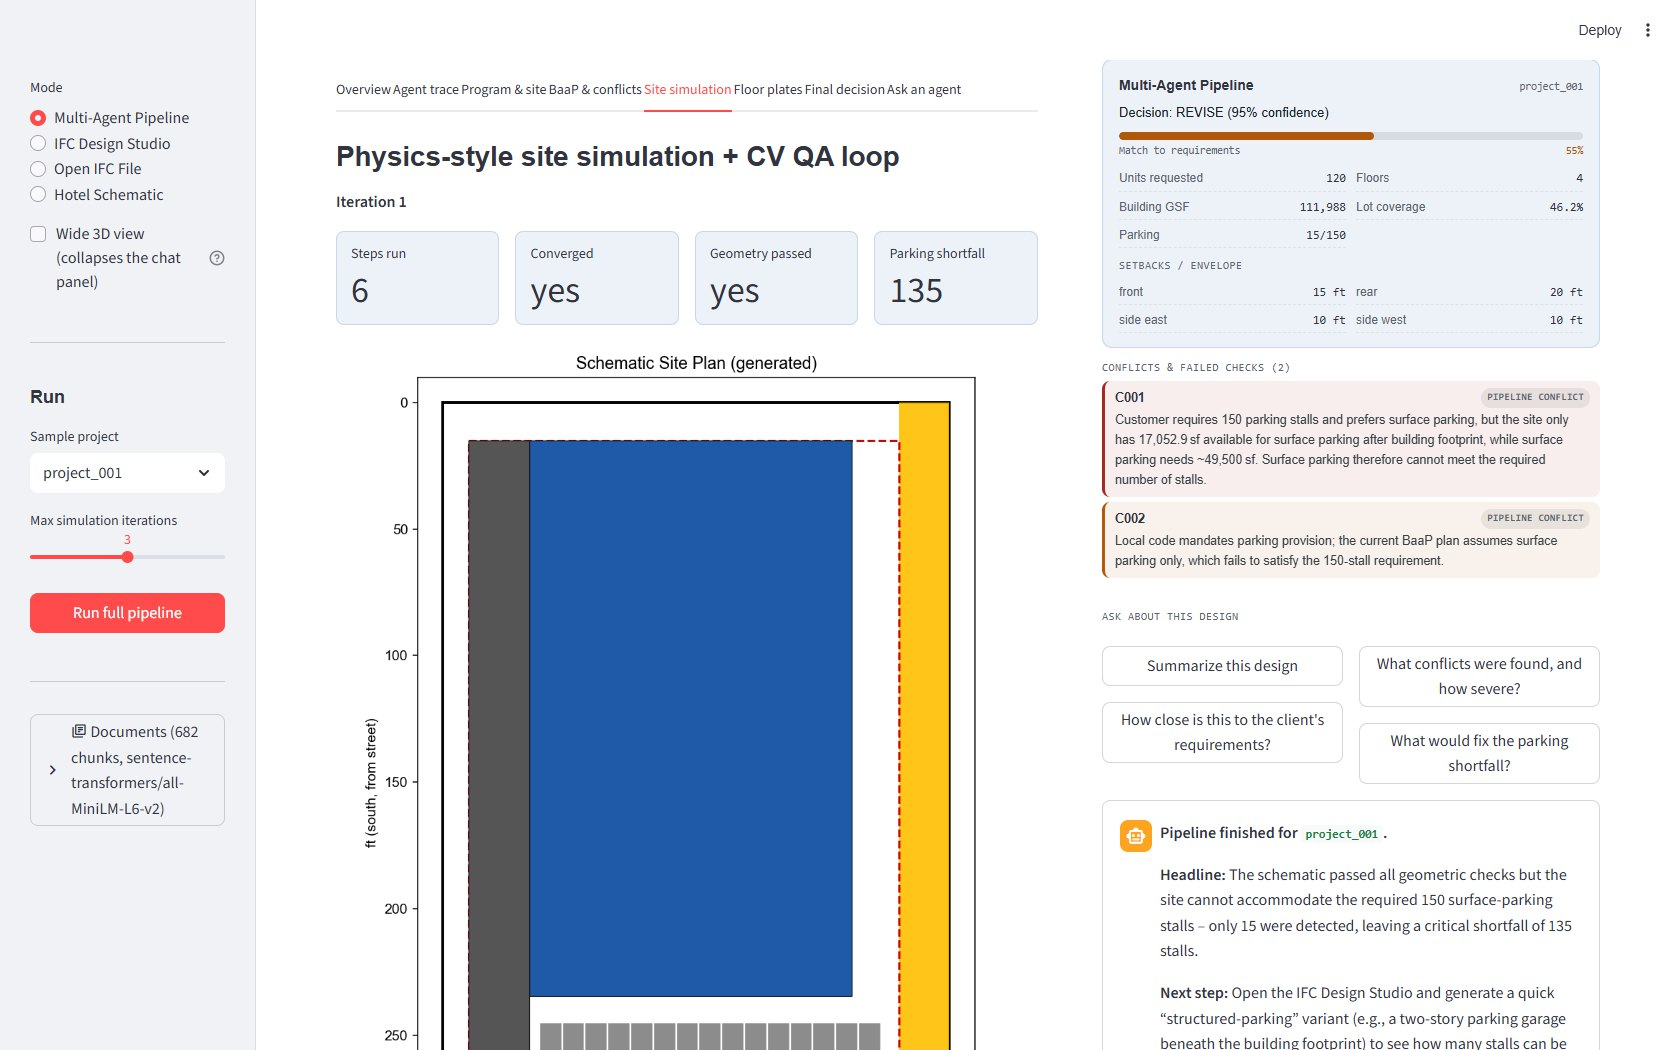
\includegraphics[width=0.92\linewidth,height=0.4\textheight,keepaspectratio]{figures/snap_07_pipeline_site_simulation}\caption*{\textbf{Screen 07.} Physics-style site simulation and the computer-vision QA of the rendered plan.}\end{figure}
\begin{figure}[H]\centering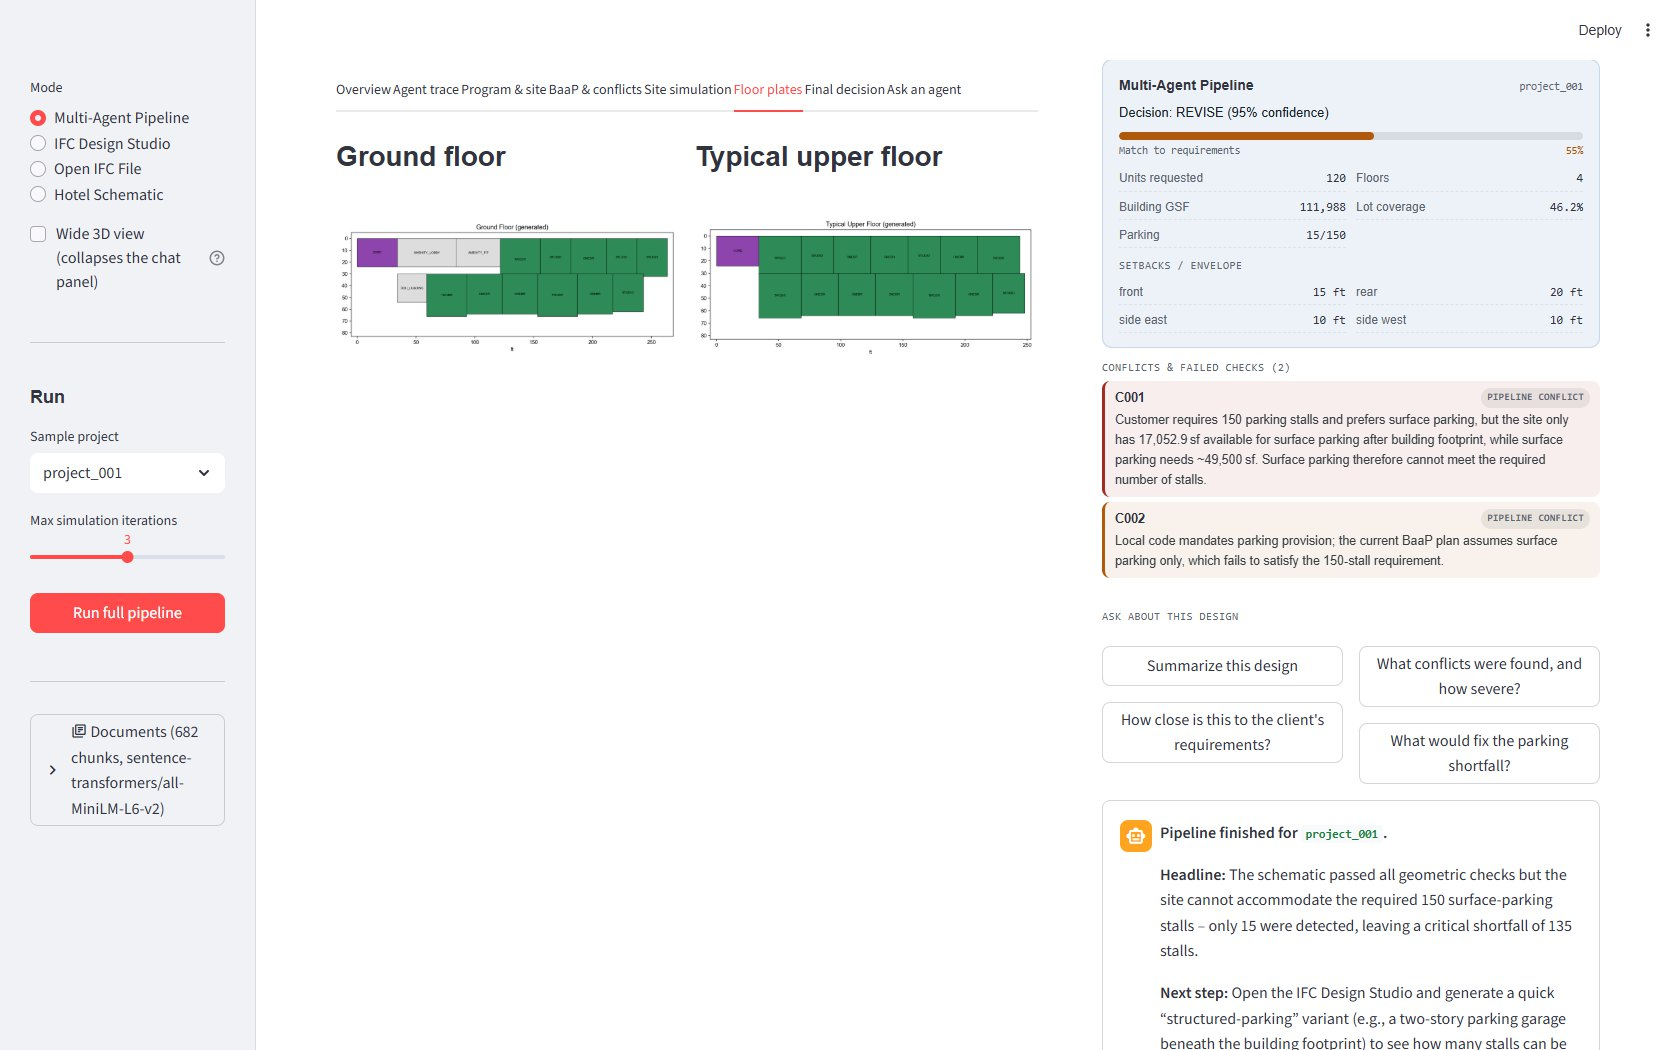
\includegraphics[width=0.92\linewidth,height=0.4\textheight,keepaspectratio]{figures/snap_08_pipeline_floor_plates}\caption*{\textbf{Screen 08.} Rule-based floor plates (ground and typical floor).}\end{figure}
\begin{figure}[H]\centering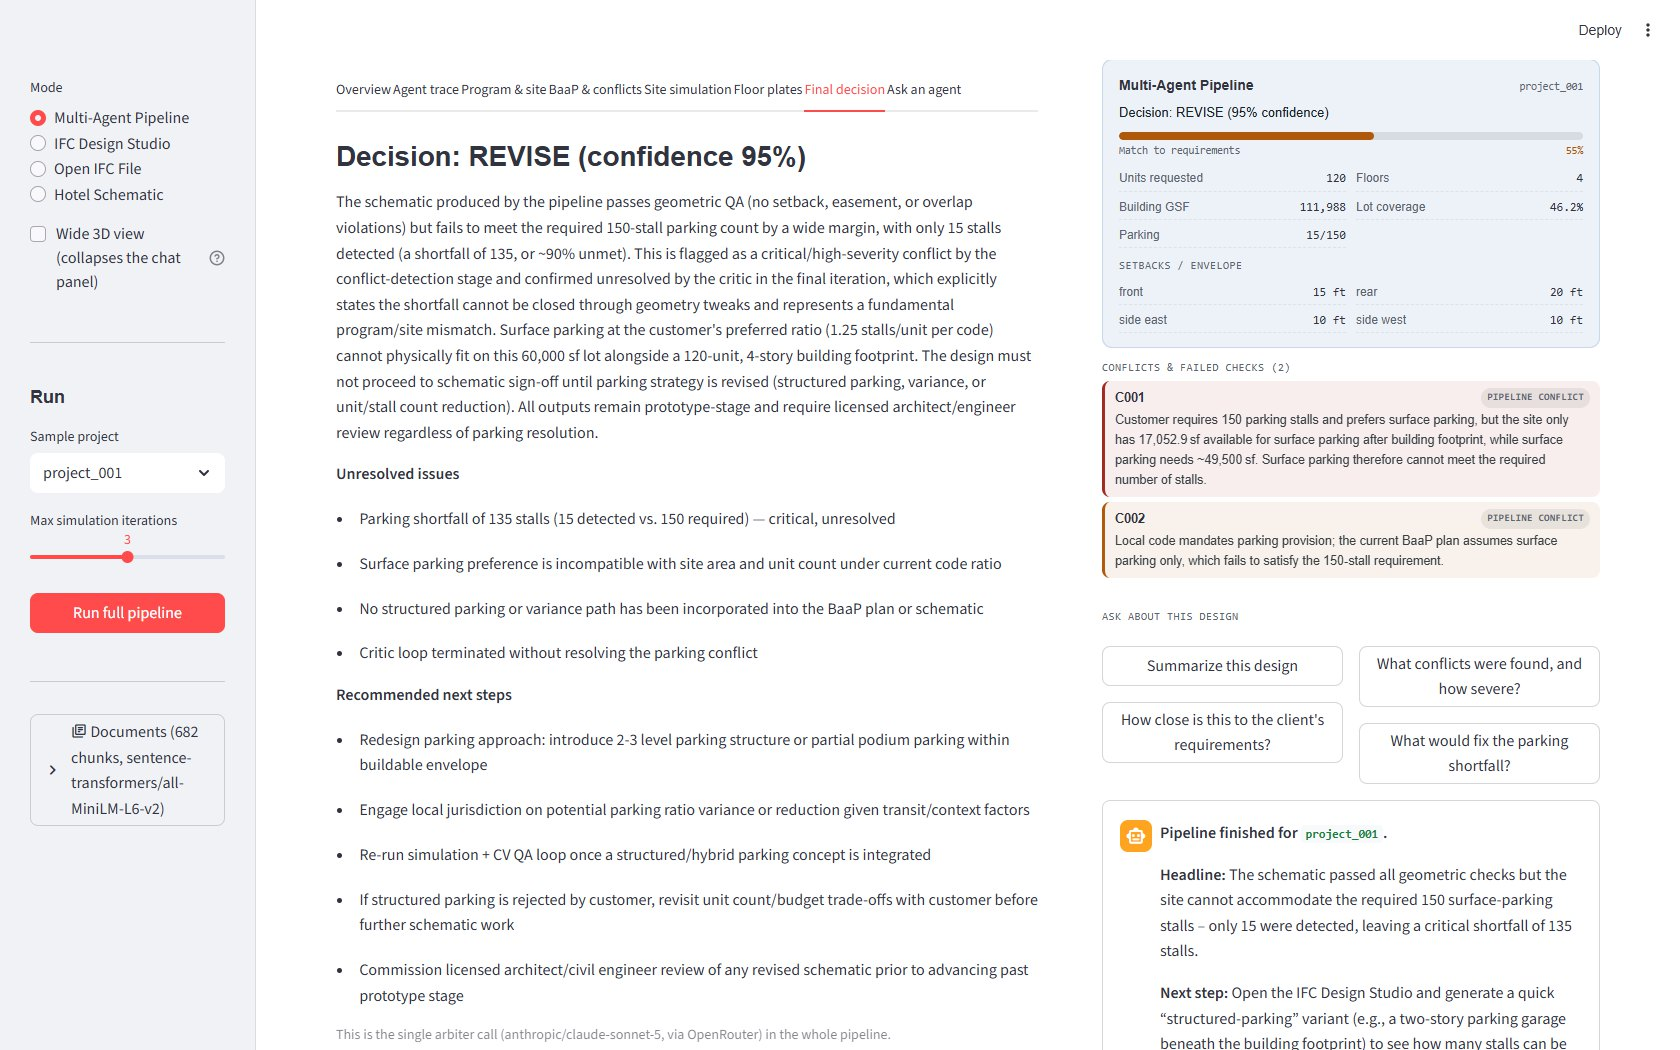
\includegraphics[width=0.92\linewidth,height=0.4\textheight,keepaspectratio]{figures/snap_09_pipeline_final_decision}\caption*{\textbf{Screen 09.} The arbiter's final decision, unresolved issues and next steps.}\end{figure}
\subsection*{IFC Design Studio}
\begin{figure}[H]\centering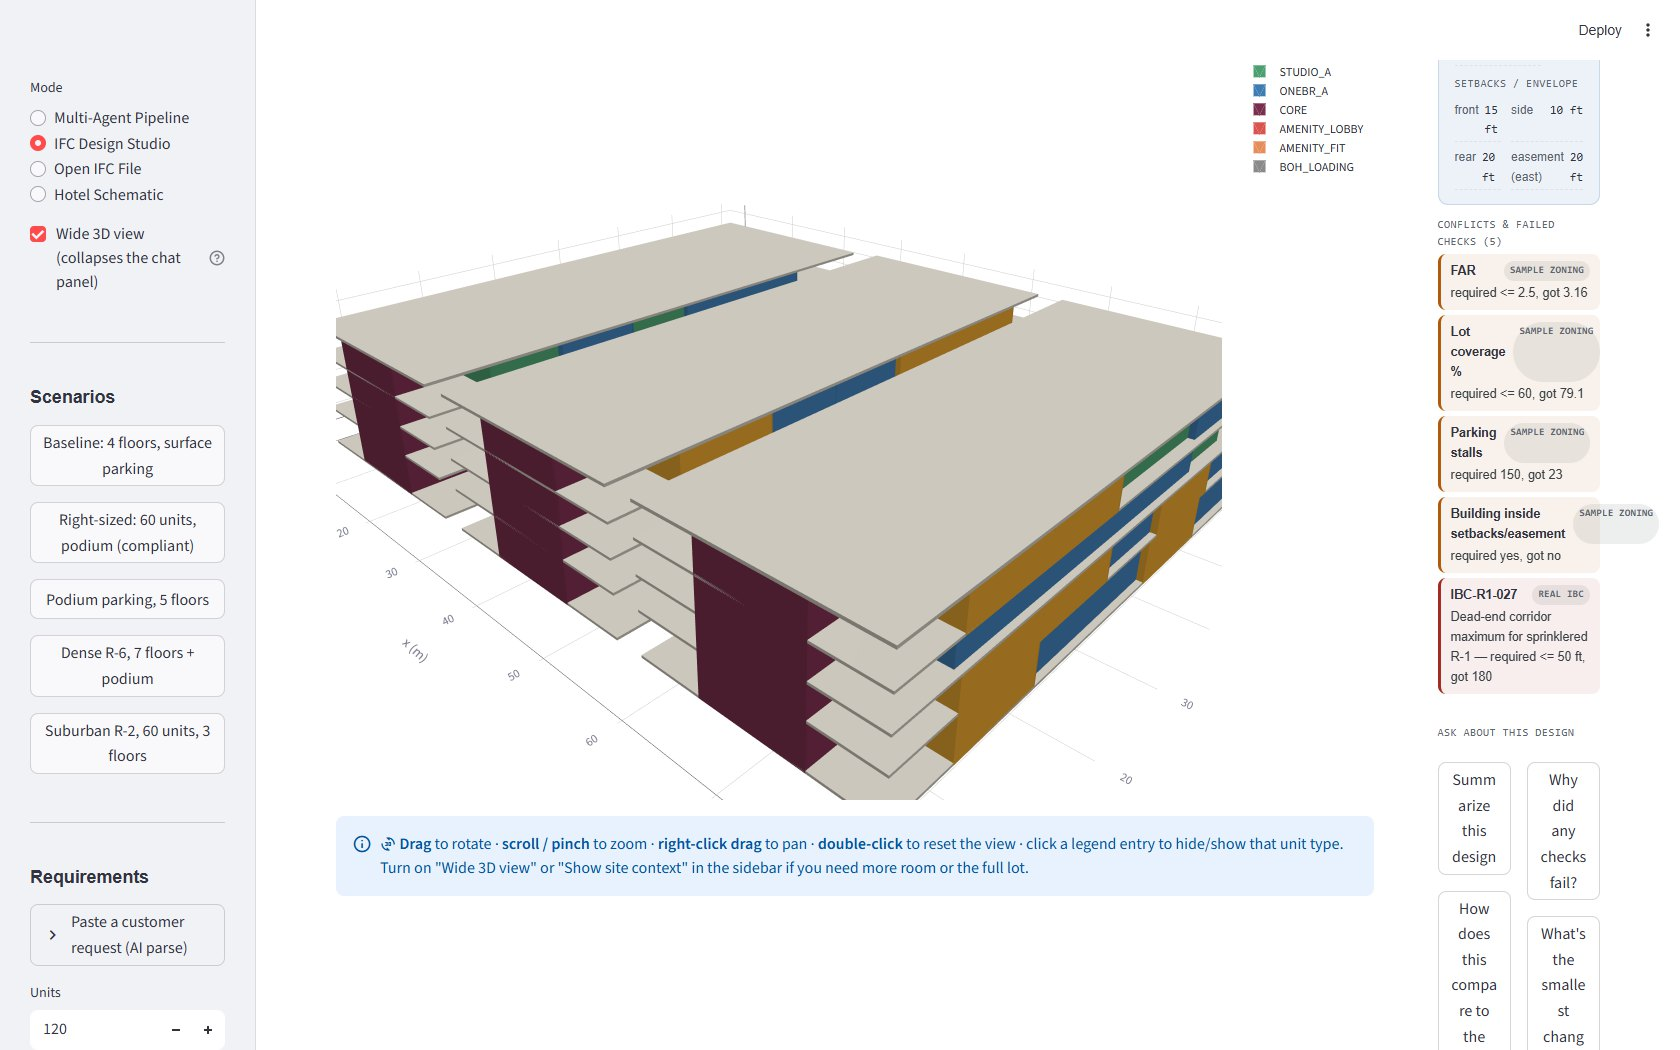
\includegraphics[width=0.92\linewidth,height=0.4\textheight,keepaspectratio]{figures/snap_10_ifc_baseline_3d_model}\caption*{\textbf{Screen 10.} IFC Design Studio, Baseline scenario (120 units, 4 floors, surface parking): the generated IFC4 model in the 3D viewer.}\end{figure}
\begin{figure}[H]\centering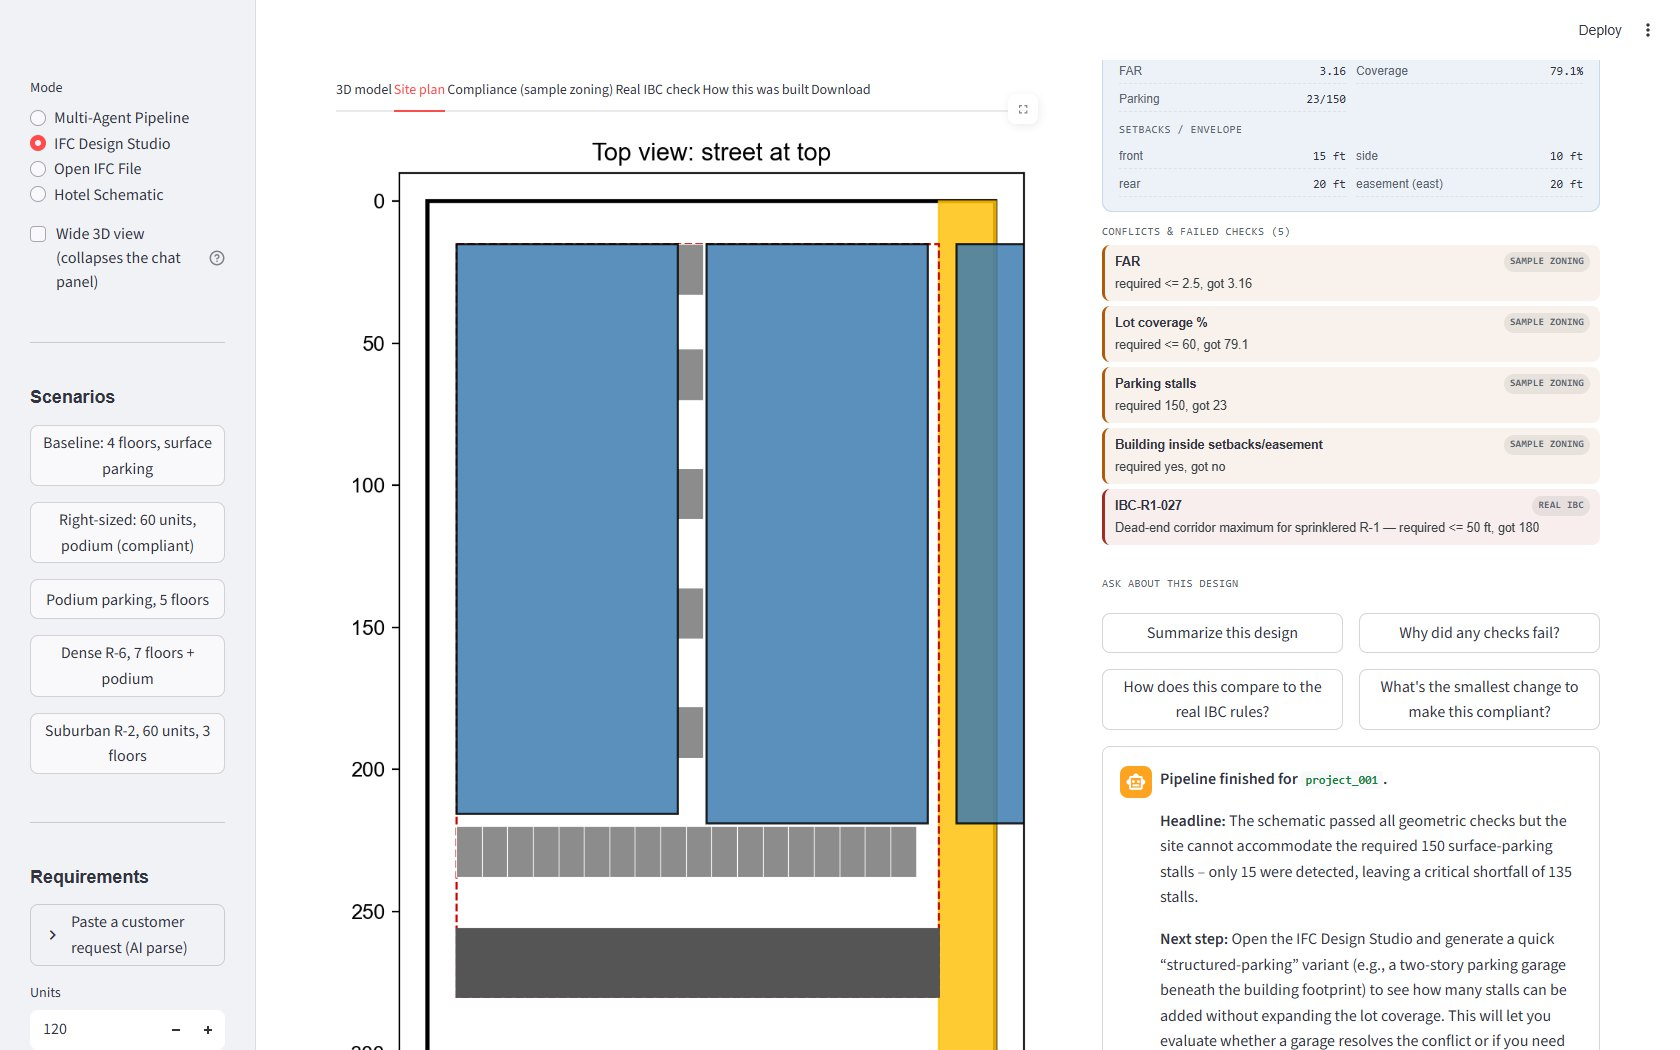
\includegraphics[width=0.92\linewidth,height=0.4\textheight,keepaspectratio]{figures/snap_11_ifc_baseline_site_plan}\caption*{\textbf{Screen 11.} Baseline site plan: building, parking, easement and fire lane on the synthetic lot.}\end{figure}
\begin{figure}[H]\centering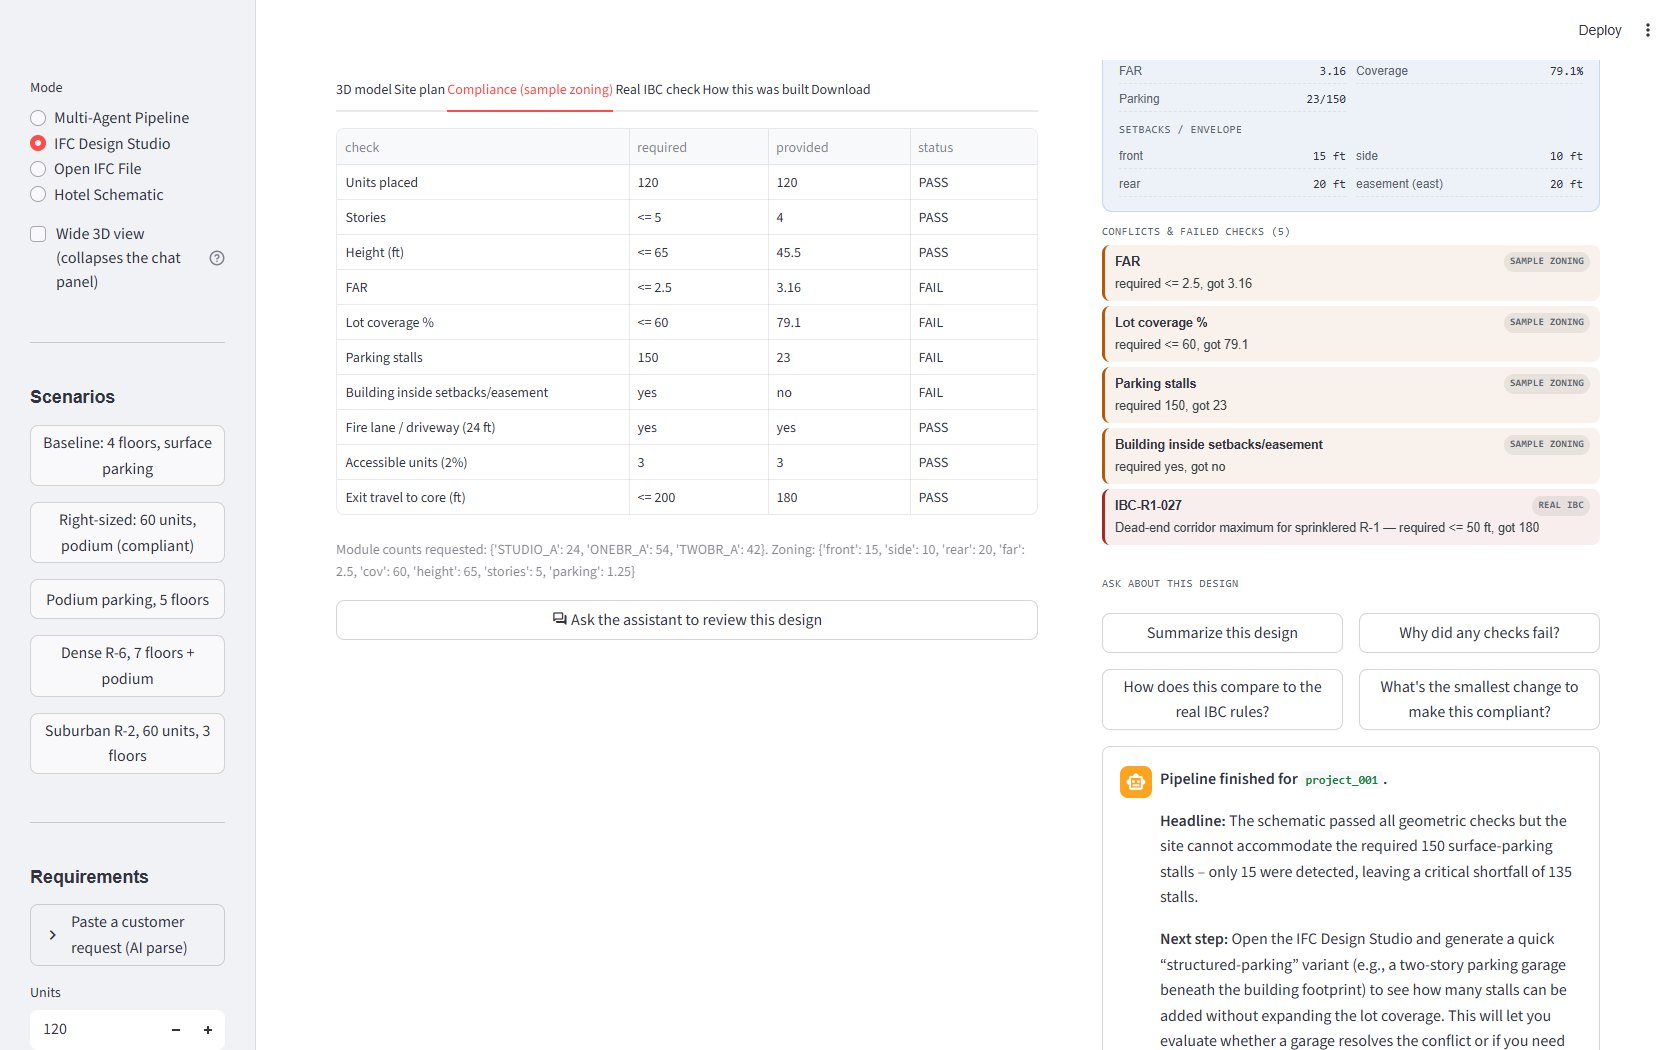
\includegraphics[width=0.92\linewidth,height=0.4\textheight,keepaspectratio]{figures/snap_12_ifc_baseline_compliance}\caption*{\textbf{Screen 12.} Baseline compliance against the ten sample-zoning checks.}\end{figure}
\begin{figure}[H]\centering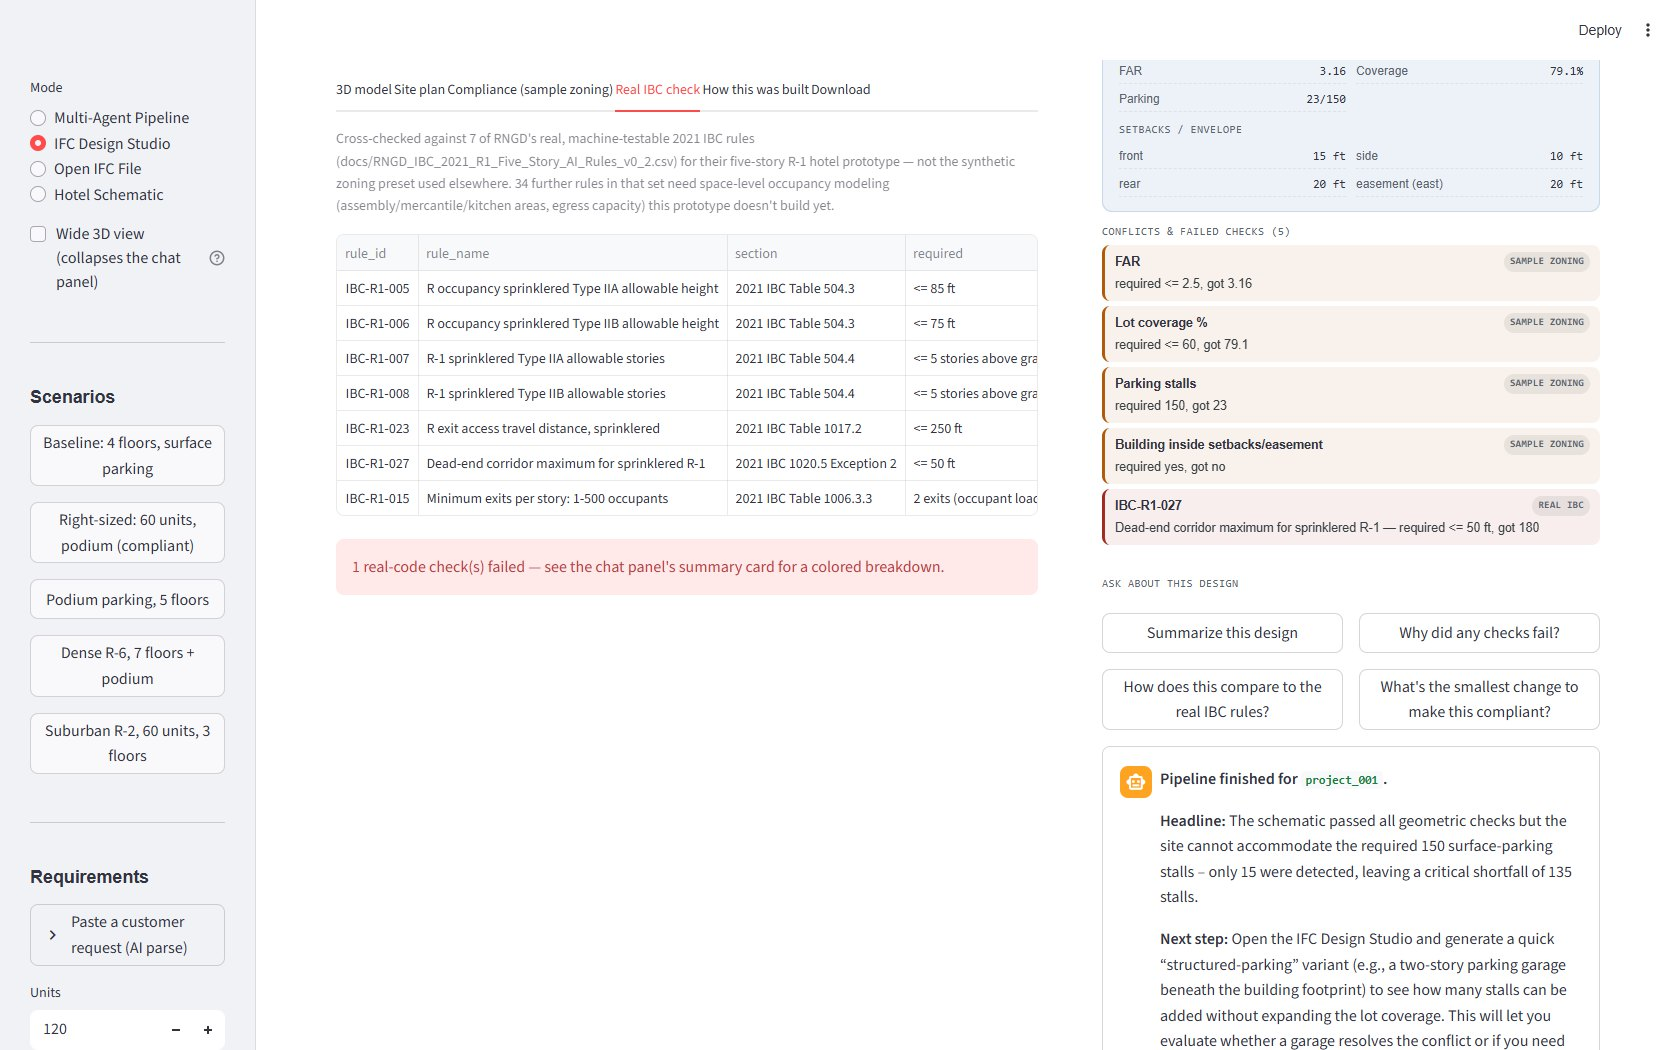
\includegraphics[width=0.92\linewidth,height=0.4\textheight,keepaspectratio]{figures/snap_13_ifc_baseline_real_ibc_check}\caption*{\textbf{Screen 13.} Baseline cross-checked against RNGD's real 2021 IBC rules.}\end{figure}
\begin{figure}[H]\centering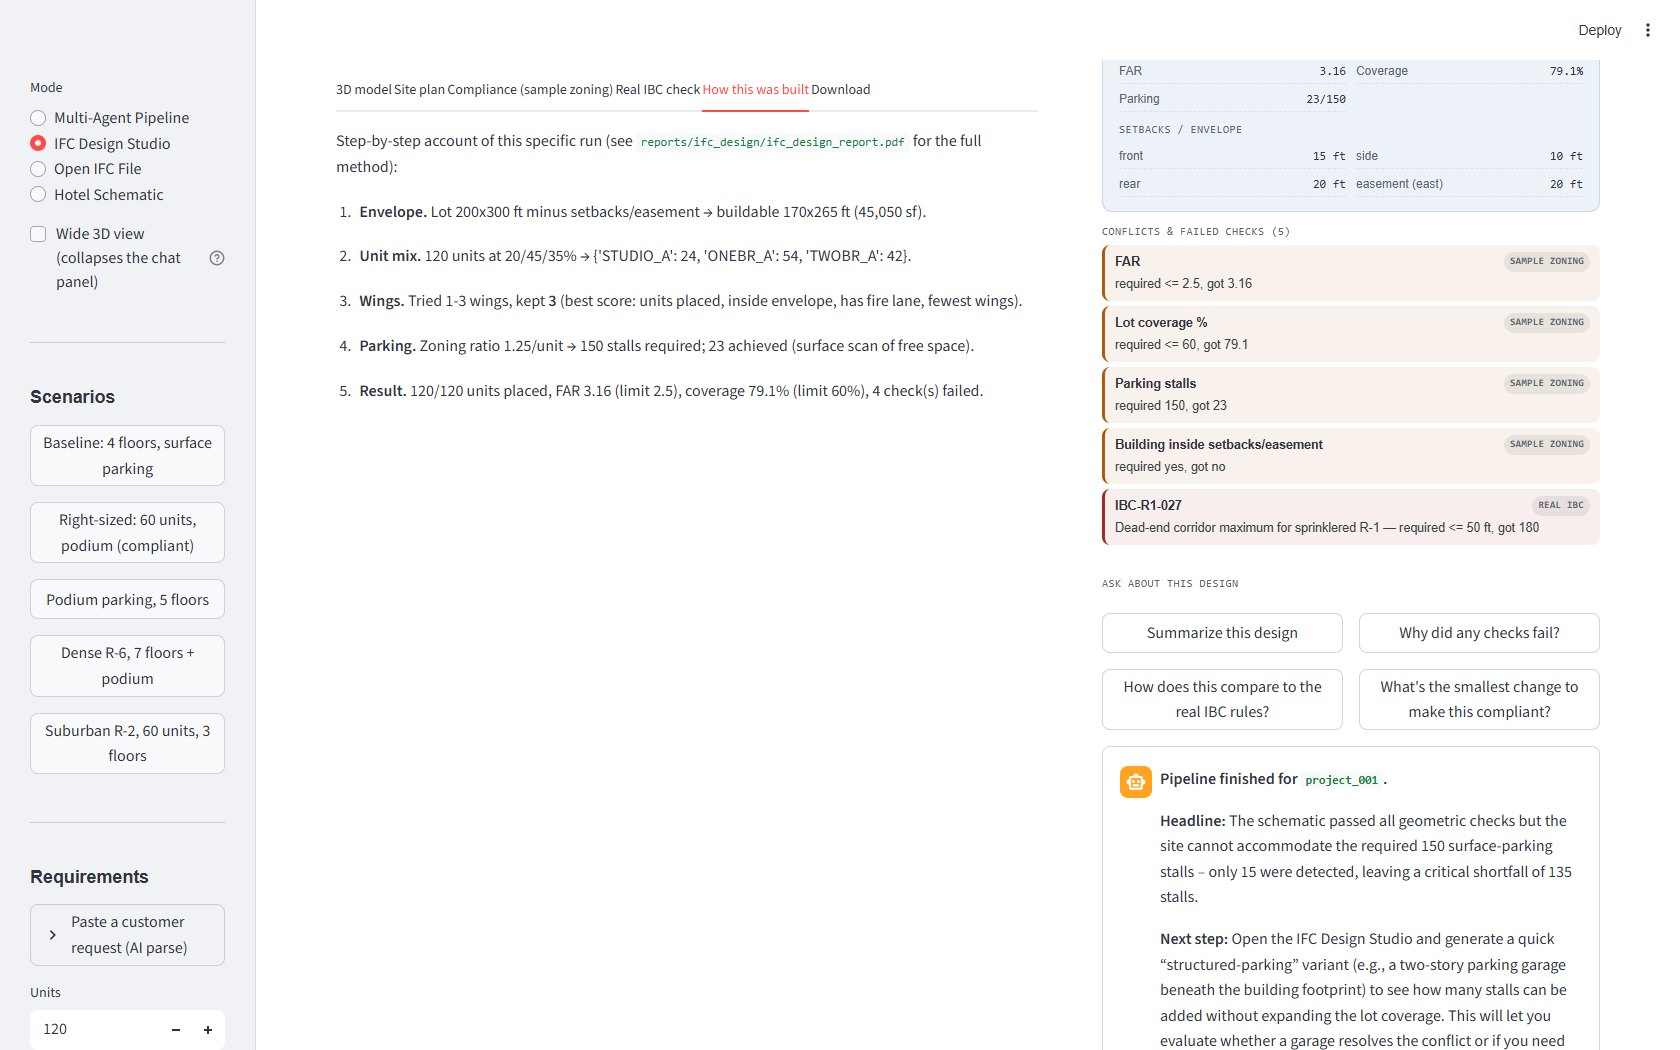
\includegraphics[width=0.92\linewidth,height=0.4\textheight,keepaspectratio]{figures/snap_14_ifc_baseline_how_this_was_built}\caption*{\textbf{Screen 14.} Step-by-step explanation of how the layout was generated.}\end{figure}
\begin{figure}[H]\centering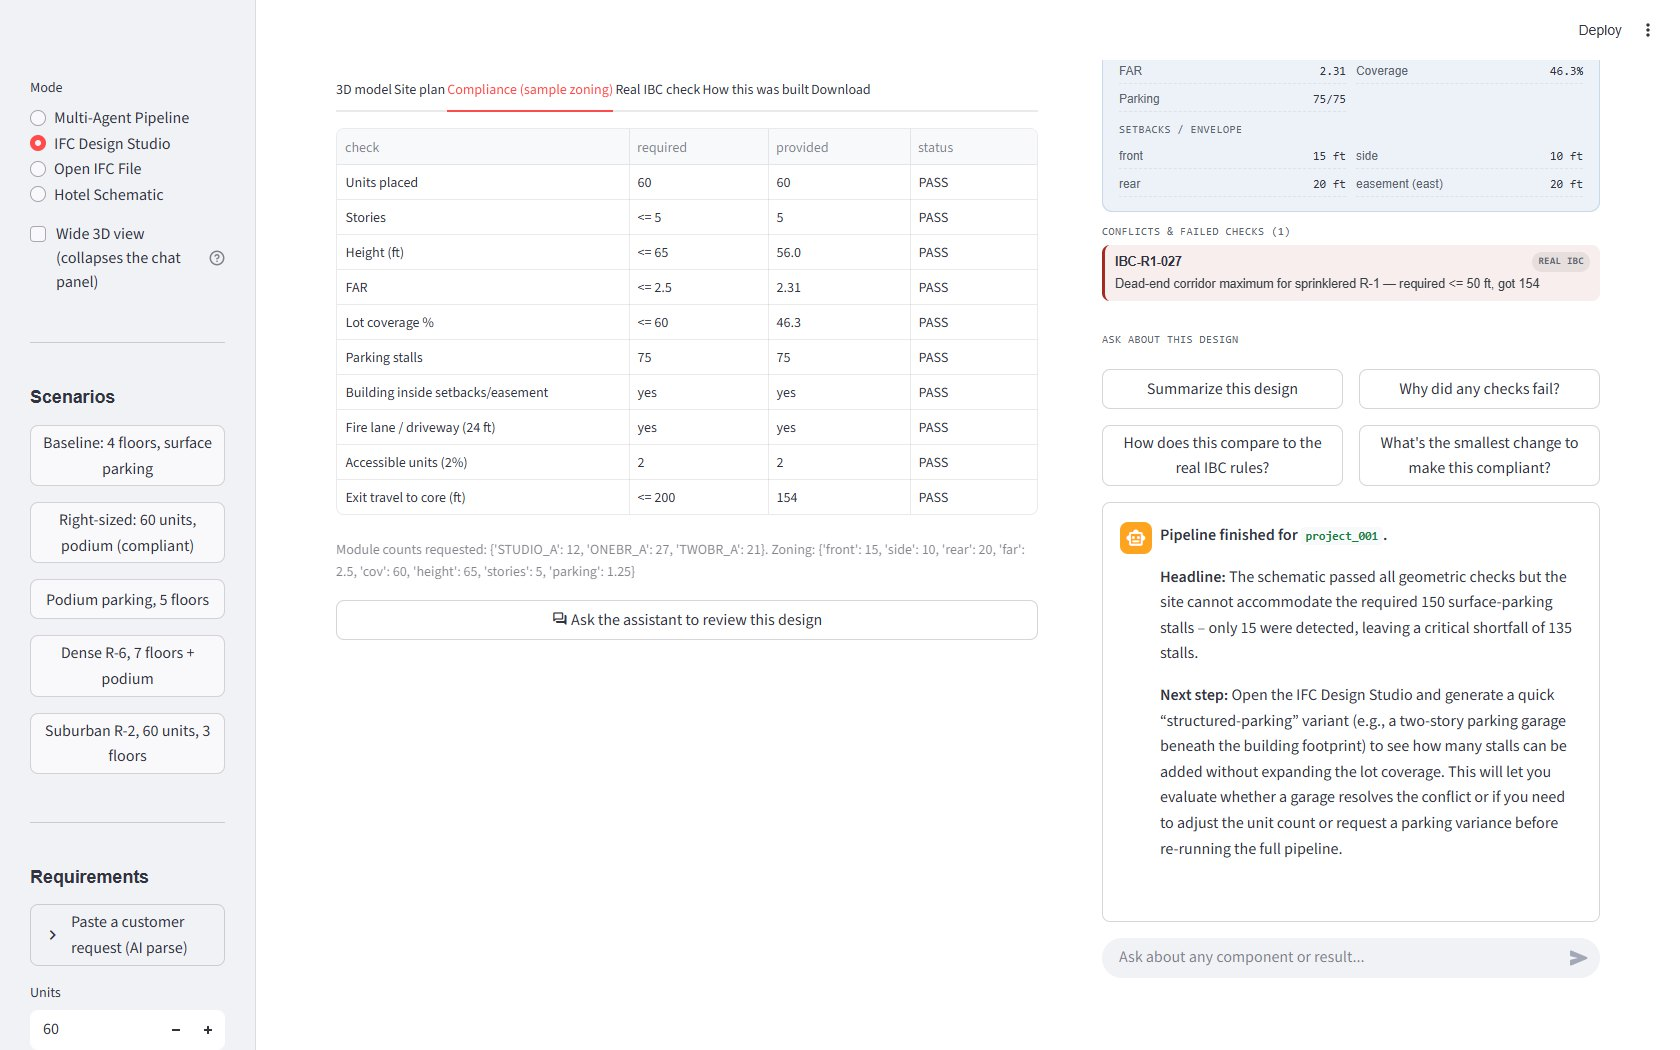
\includegraphics[width=0.92\linewidth,height=0.4\textheight,keepaspectratio]{figures/snap_15_ifc_rightsized_compliance}\caption*{\textbf{Screen 15.} Right-sized scenario (60 units, podium parking): the compliance checks after the fix.}\end{figure}
\begin{figure}[H]\centering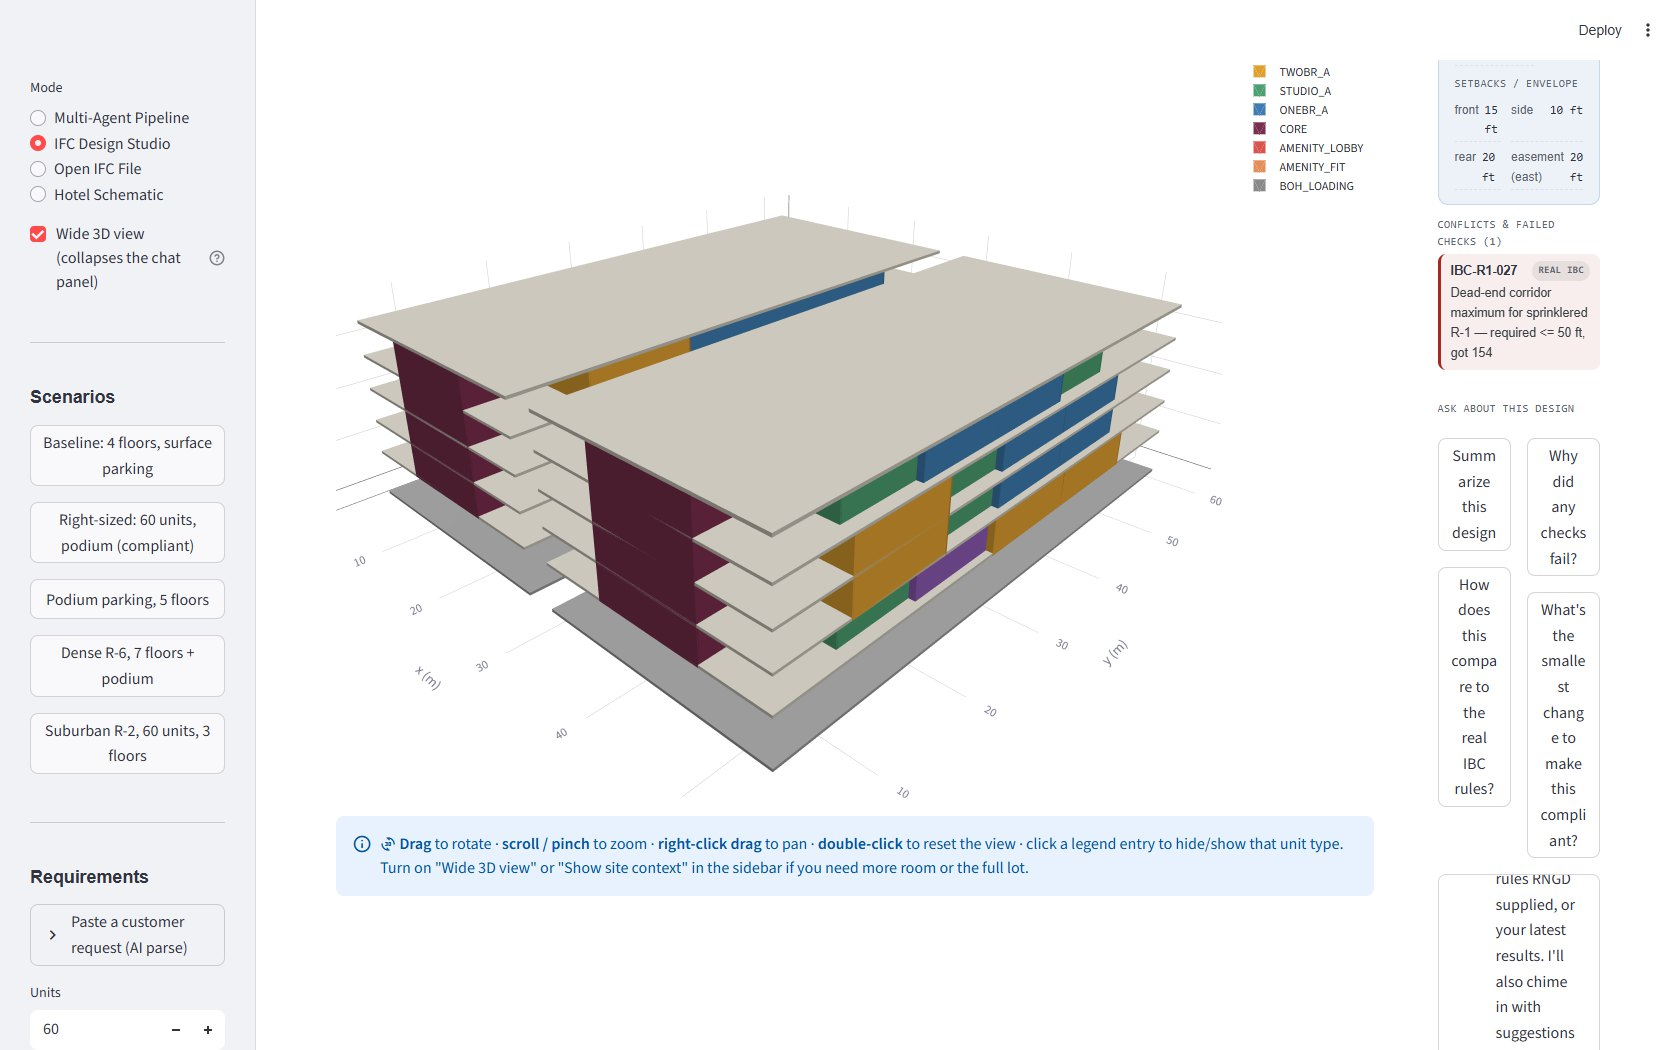
\includegraphics[width=0.92\linewidth,height=0.4\textheight,keepaspectratio]{figures/snap_16_ifc_rightsized_3d}\caption*{\textbf{Screen 16.} Right-sized scenario in 3D.}\end{figure}
\subsection*{Open IFC File}
\begin{figure}[H]\centering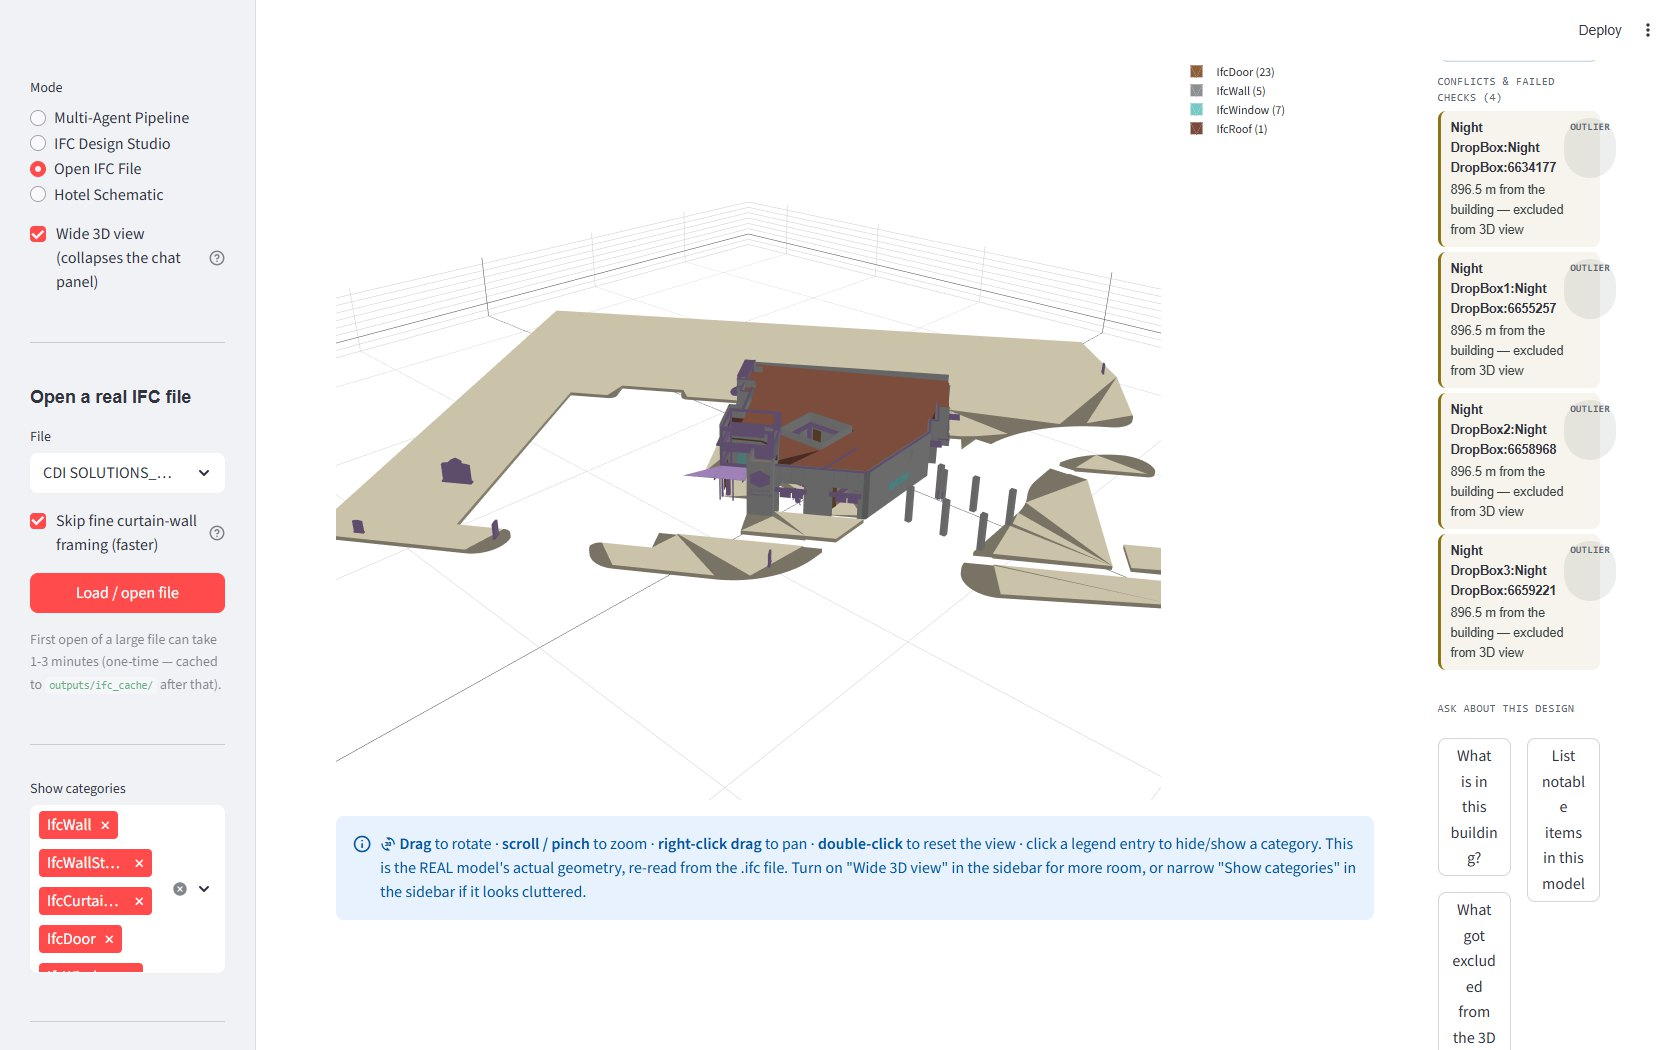
\includegraphics[width=0.92\linewidth,height=0.4\textheight,keepaspectratio]{figures/snap_17_explorer_3d_model}\caption*{\textbf{Screen 17.} A real IFC file (CDI Solutions, Metairie Bank, IFC2X3, 89 MB) recentred and shown in 3D.}\end{figure}
\begin{figure}[H]\centering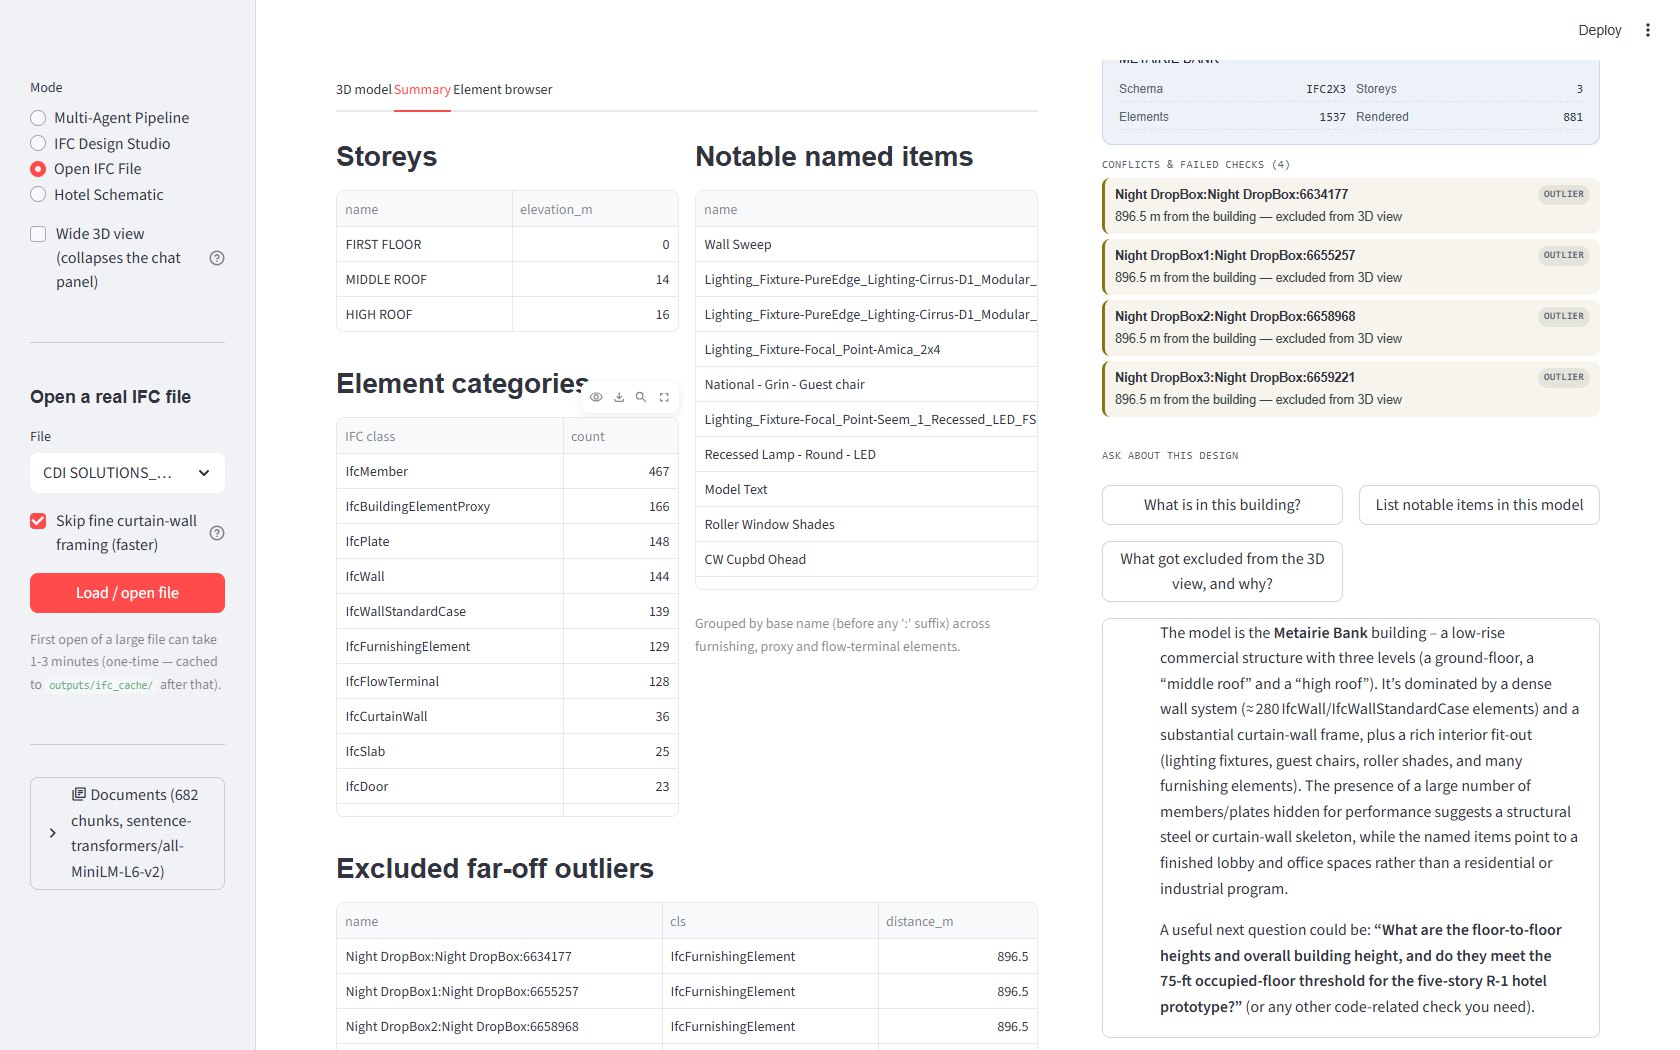
\includegraphics[width=0.92\linewidth,height=0.4\textheight,keepaspectratio]{figures/snap_18_explorer_summary}\caption*{\textbf{Screen 18.} What is in the real model: schema, storeys and element counts by IFC class.}\end{figure}
\begin{figure}[H]\centering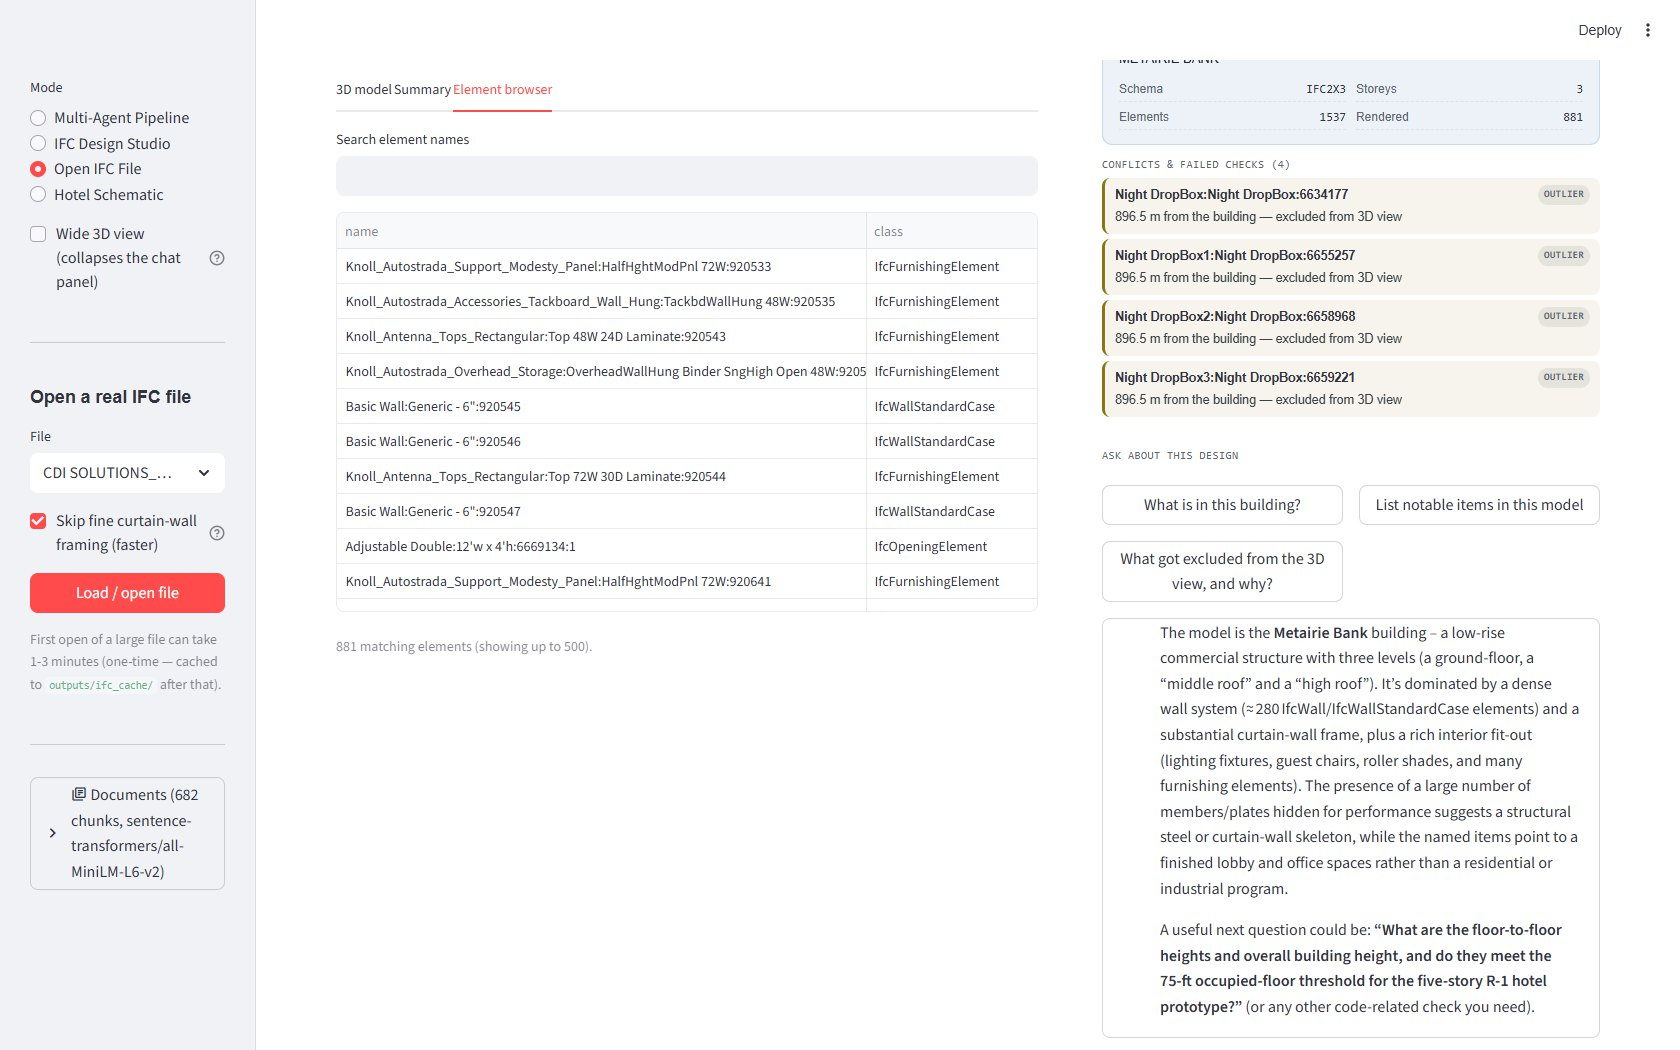
\includegraphics[width=0.92\linewidth,height=0.4\textheight,keepaspectratio]{figures/snap_19_explorer_element_browser}\caption*{\textbf{Screen 19.} Searchable list of the model's elements.}\end{figure}
\subsection*{Hotel Schematic}
\begin{figure}[H]\centering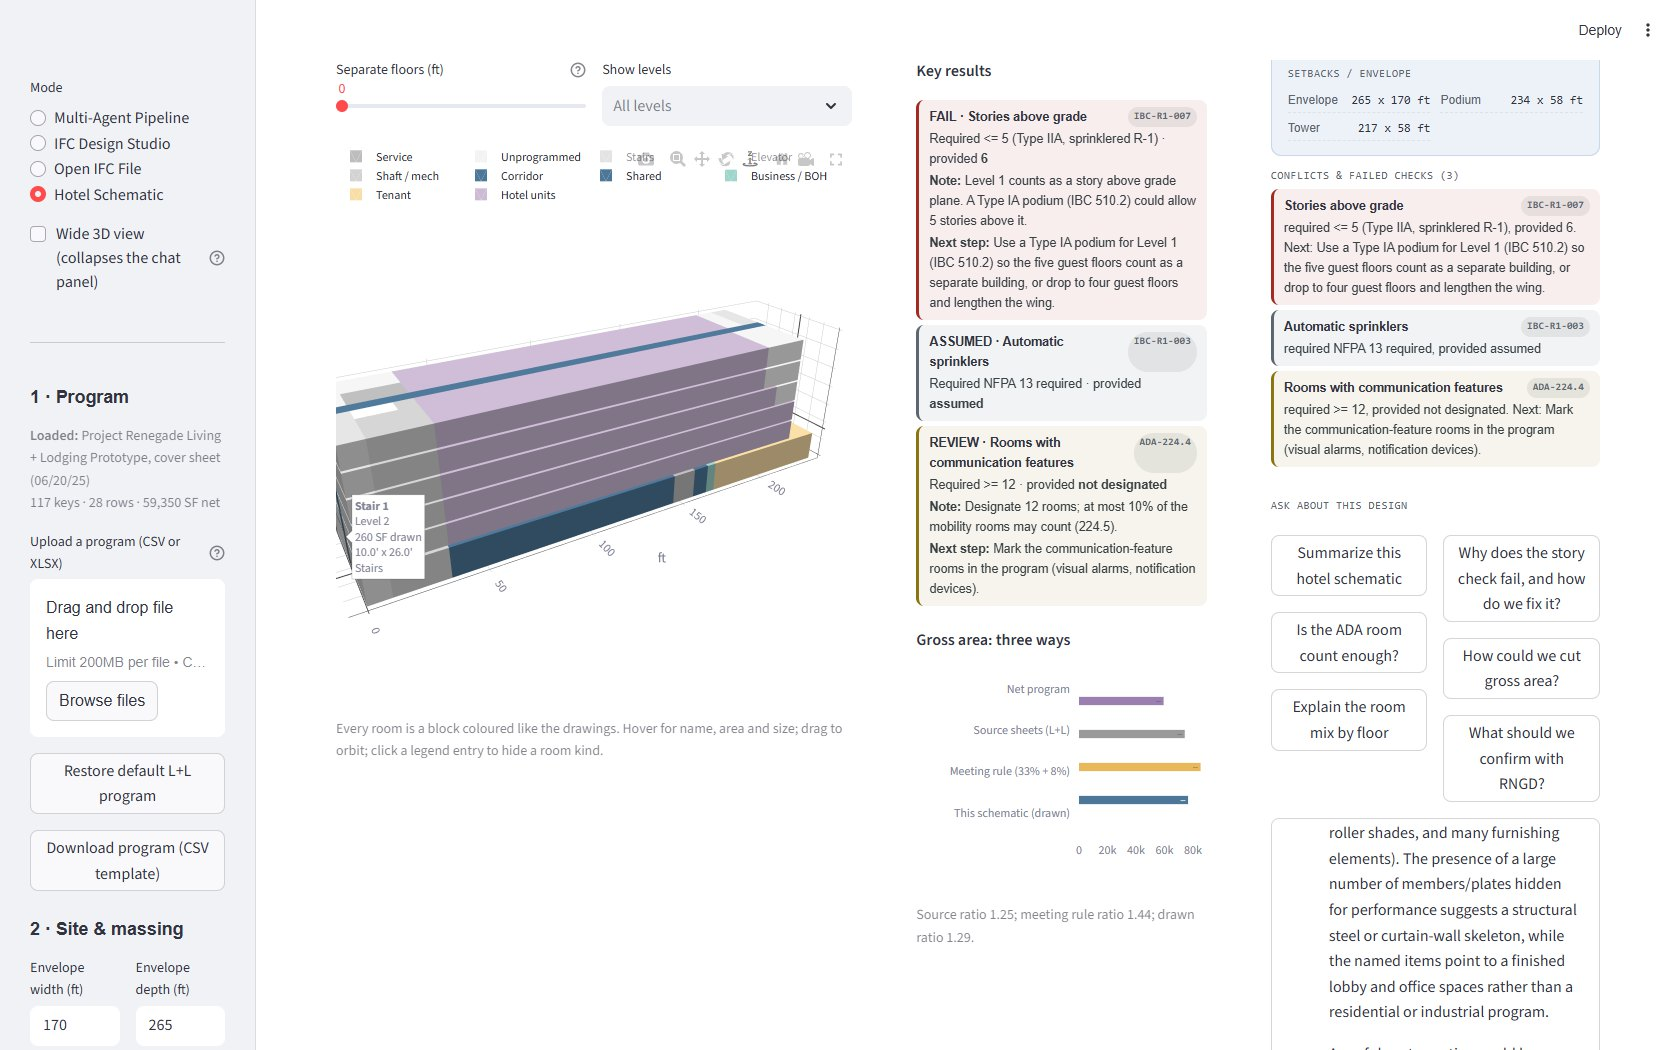
\includegraphics[width=0.92\linewidth,height=0.4\textheight,keepaspectratio]{figures/snap_20_hotel_overview}\caption*{\textbf{Screen 20.} Hotel Schematic workspace: KPI tiles, the room-by-room 3D model and the key results with suggested fixes.}\end{figure}
\begin{figure}[H]\centering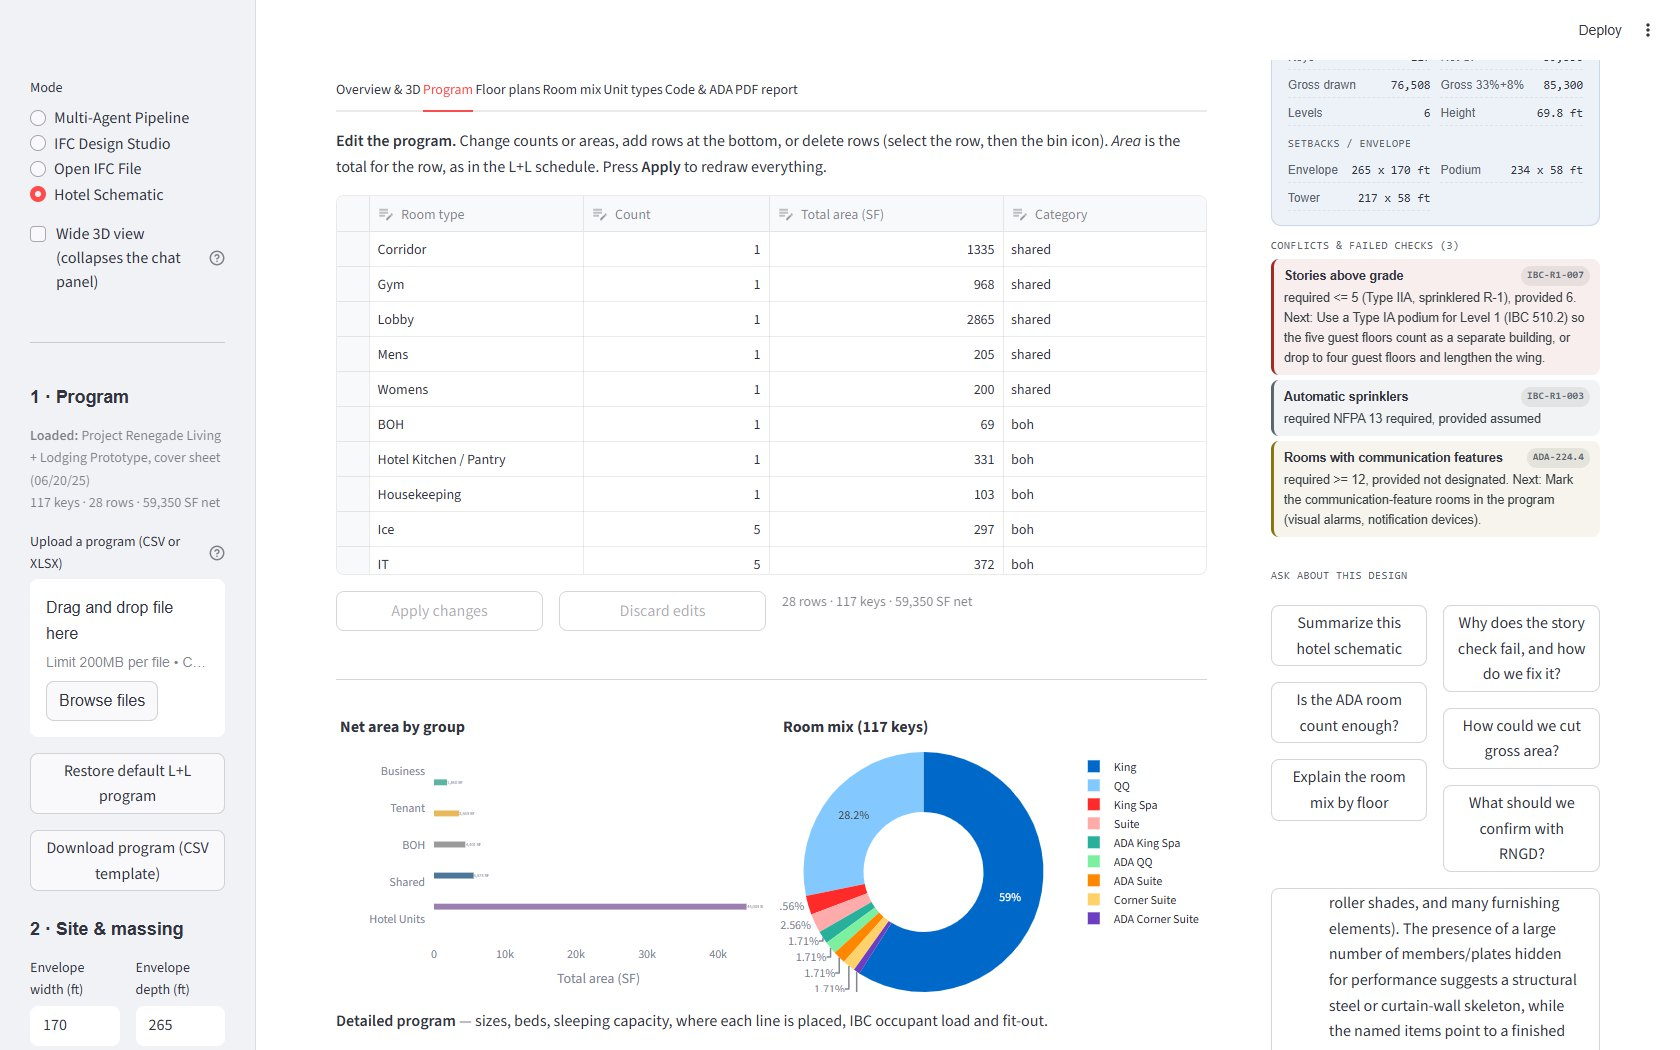
\includegraphics[width=0.92\linewidth,height=0.4\textheight,keepaspectratio]{figures/snap_21_hotel_program}\caption*{\textbf{Screen 21.} The editable program (Project Renegade L+L space allocation, 28 rows) with area and room-mix charts.}\end{figure}
\begin{figure}[H]\centering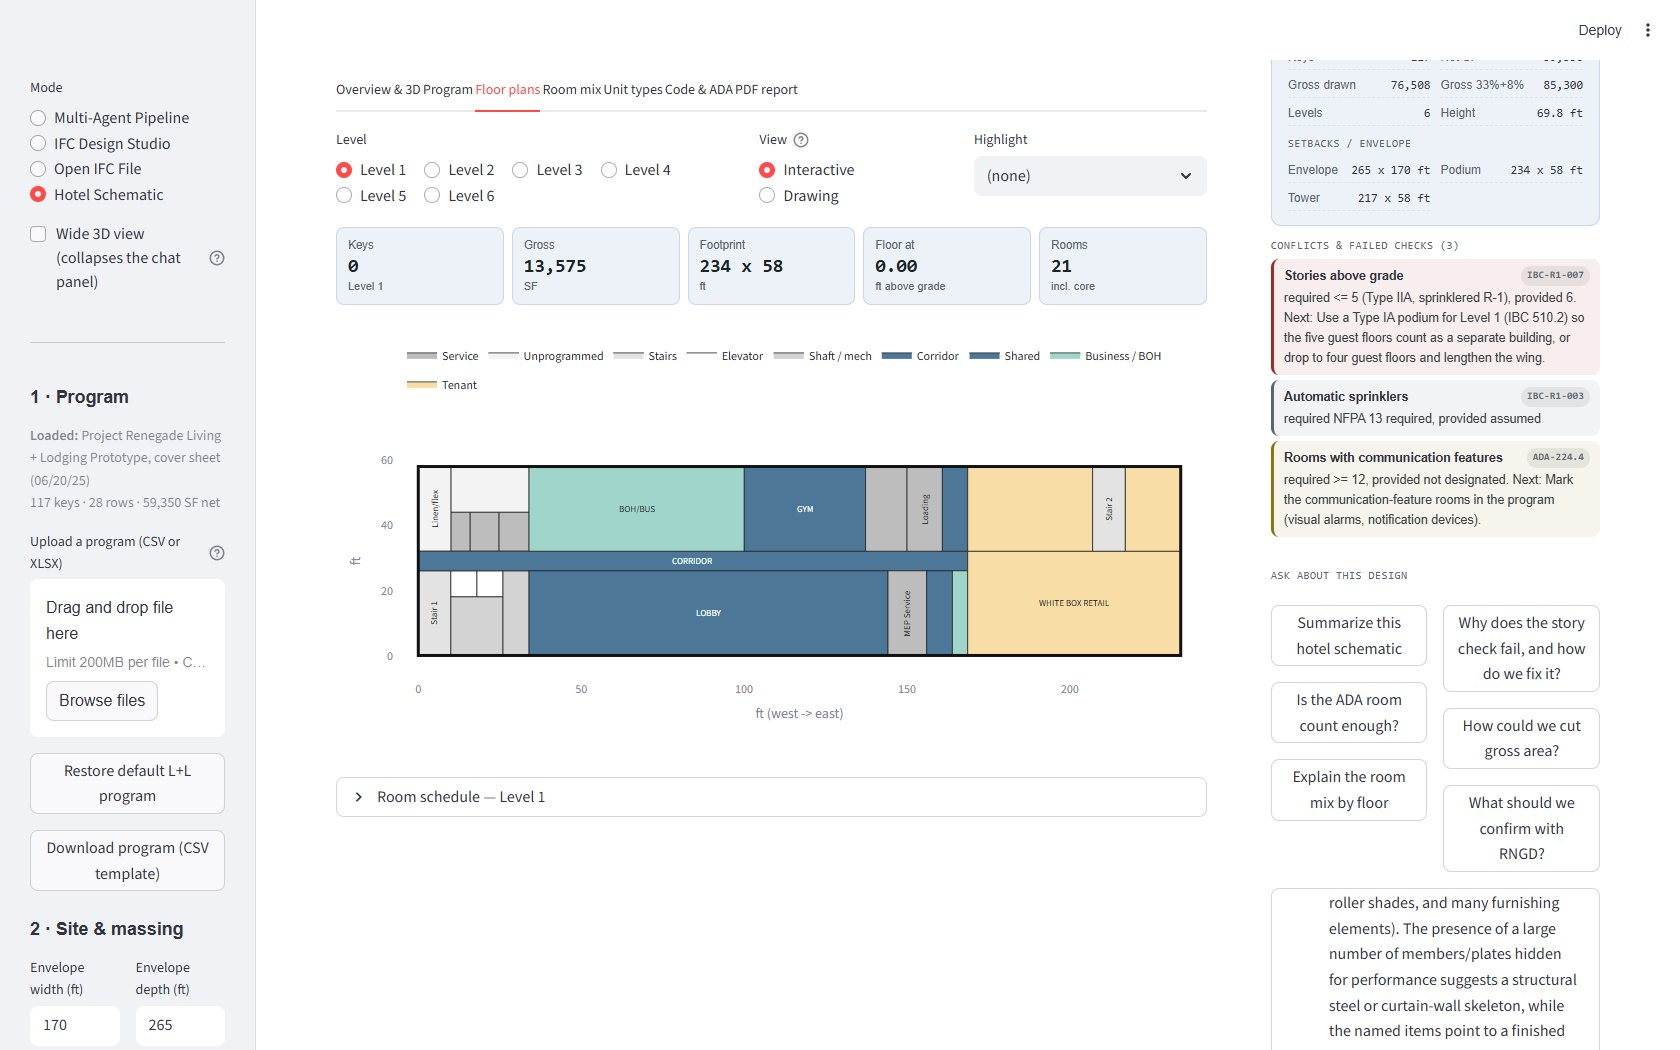
\includegraphics[width=0.92\linewidth,height=0.4\textheight,keepaspectratio]{figures/snap_22_hotel_floor}\caption*{\textbf{Screen 22.} Interactive floor plan of Level 1 (hover shows each room's area and size).}\end{figure}
\begin{figure}[H]\centering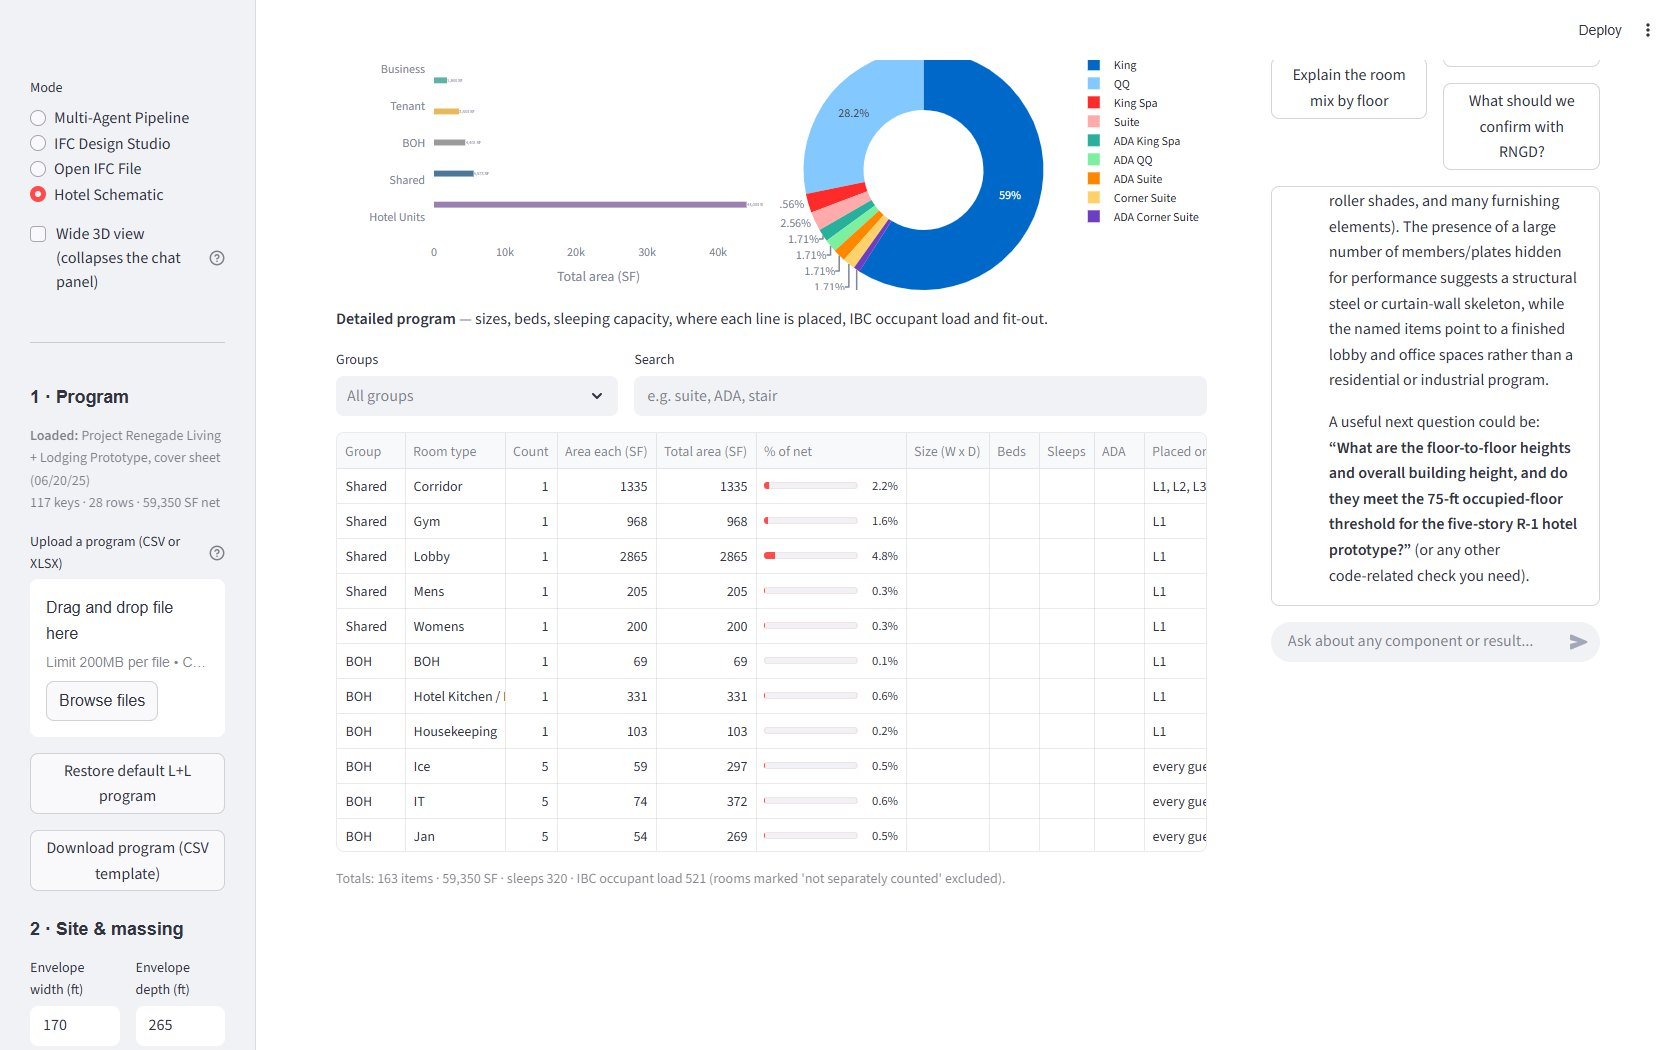
\includegraphics[width=0.92\linewidth,height=0.4\textheight,keepaspectratio]{figures/snap_23_hotel_program_detail}\caption*{\textbf{Screen 23.} Detailed program: per-room size, beds, sleeping capacity, placement, IBC occupant load and fit-out.}\end{figure}
\begin{figure}[H]\centering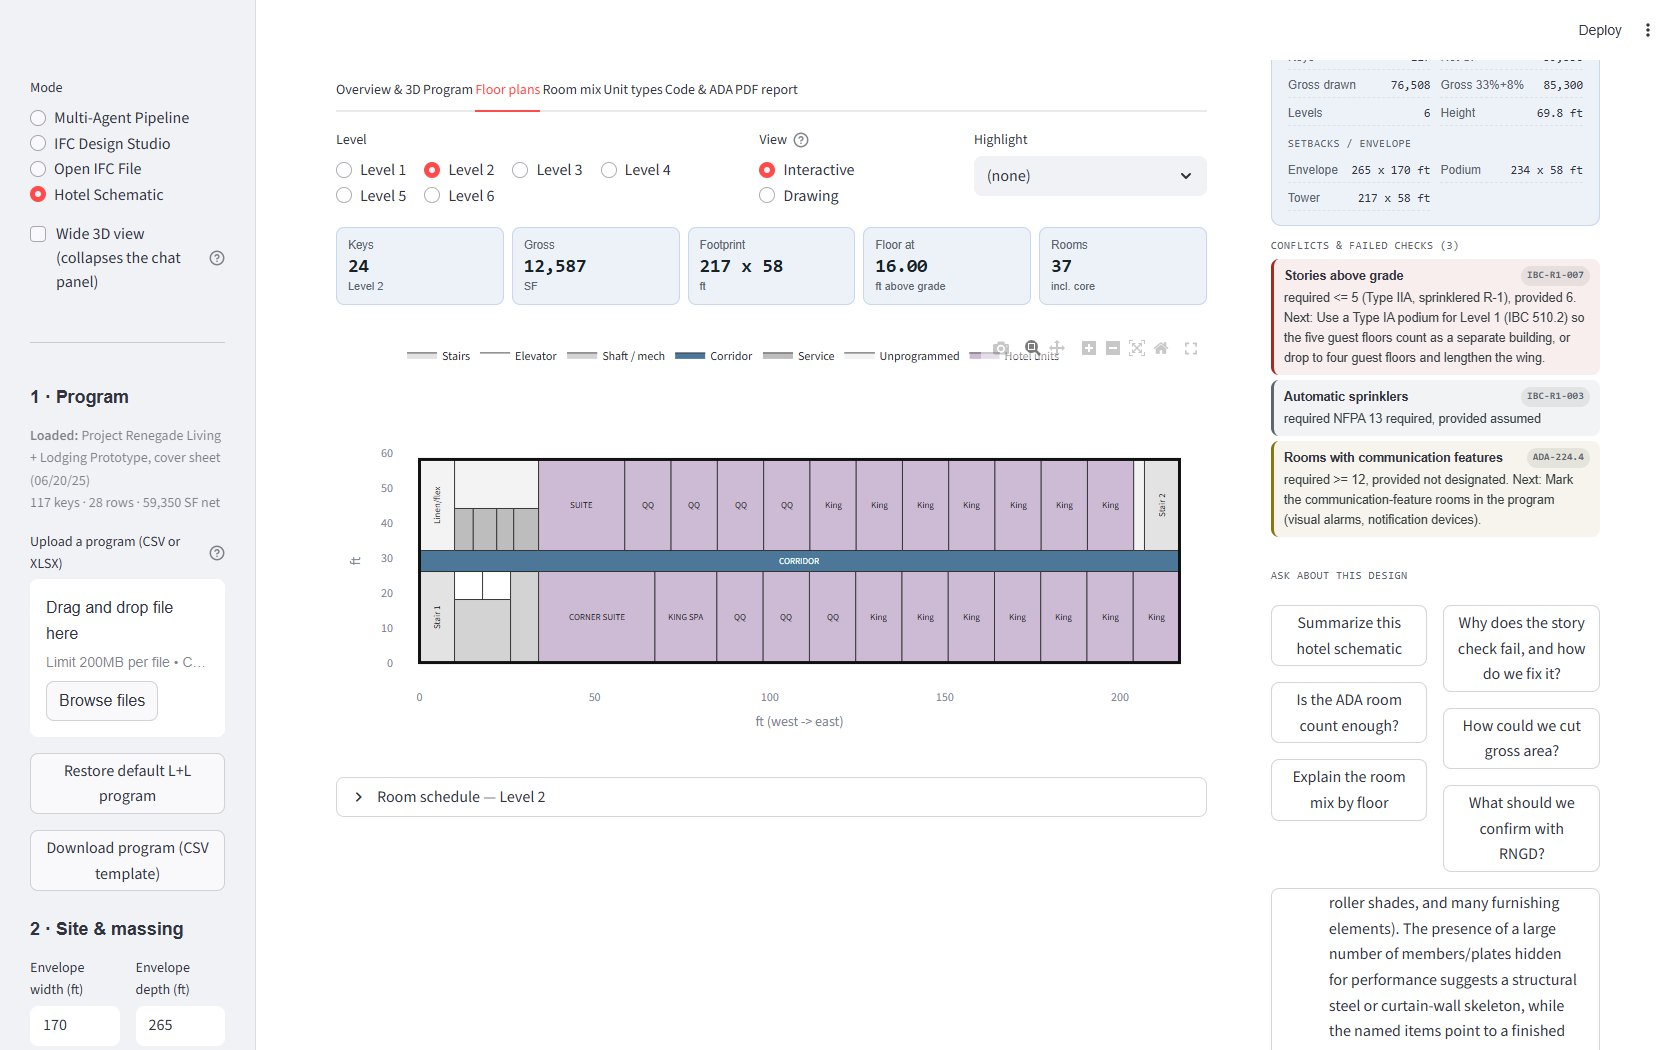
\includegraphics[width=0.92\linewidth,height=0.4\textheight,keepaspectratio]{figures/snap_24_hotel_plan_level2}\caption*{\textbf{Screen 24.} Interactive plan of Level 2, a typical guest floor (24 keys).}\end{figure}
\begin{figure}[H]\centering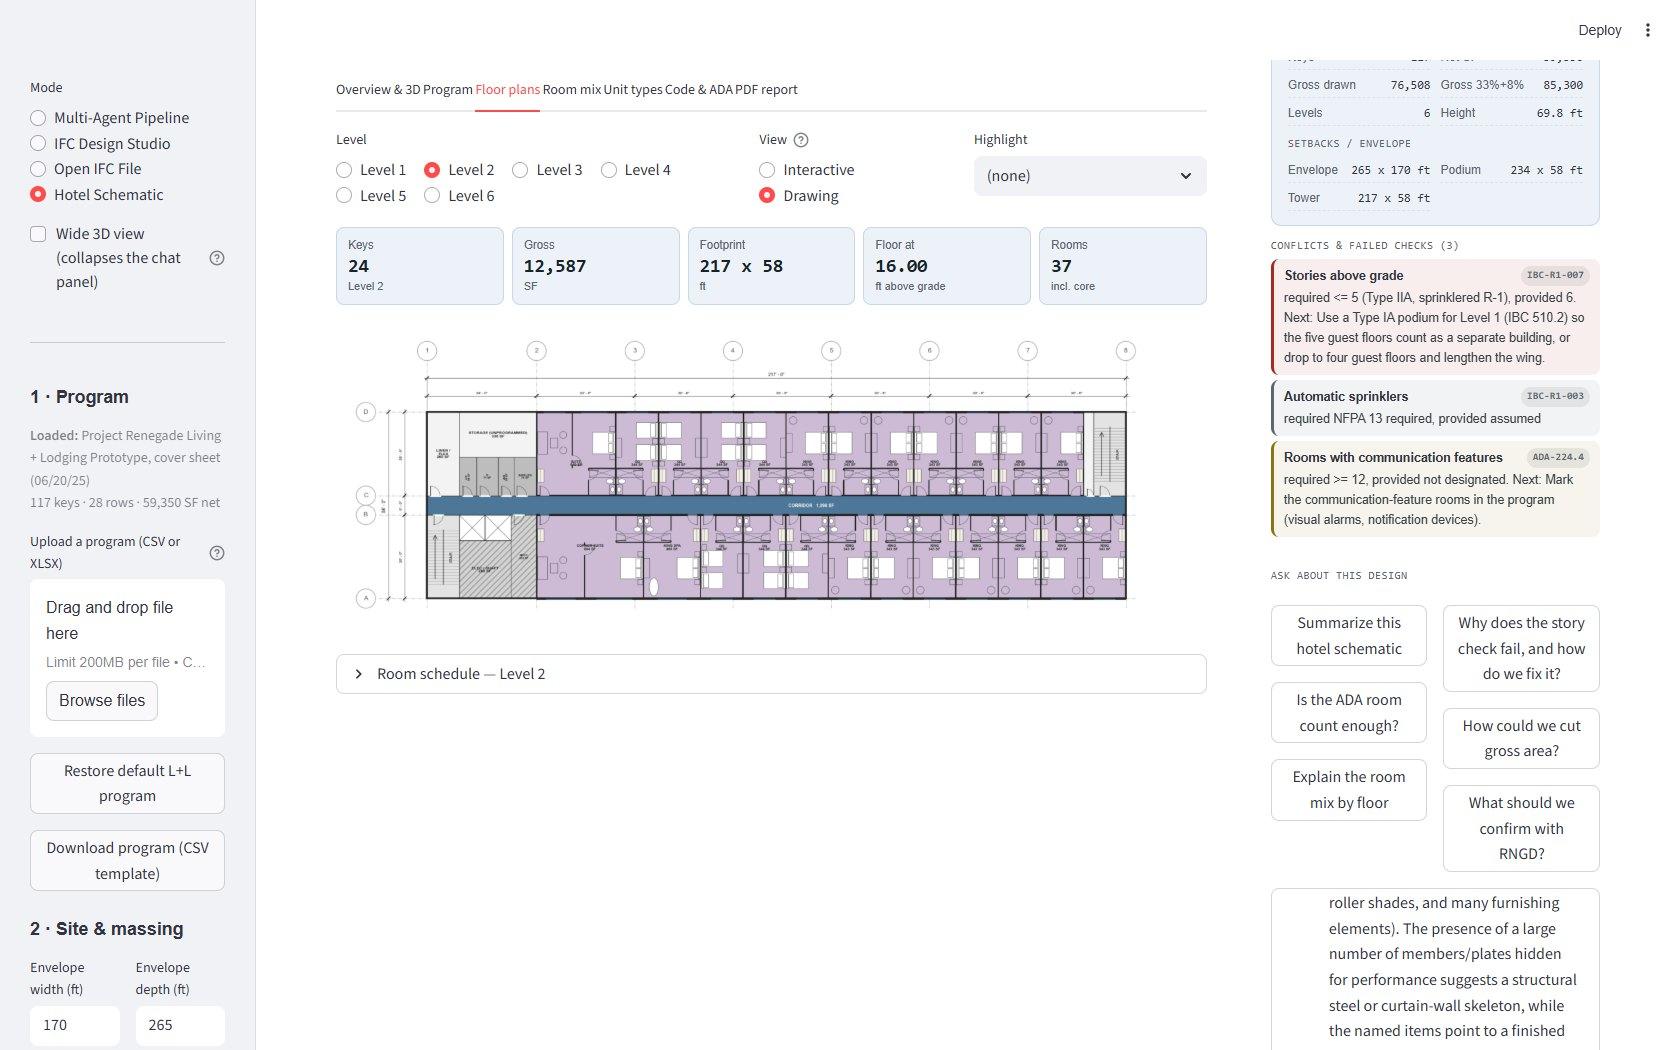
\includegraphics[width=0.92\linewidth,height=0.4\textheight,keepaspectratio]{figures/snap_25_hotel_plan_drawing}\caption*{\textbf{Screen 25.} The same level in drawing style (as used on the PDF sheets).}\end{figure}
\begin{figure}[H]\centering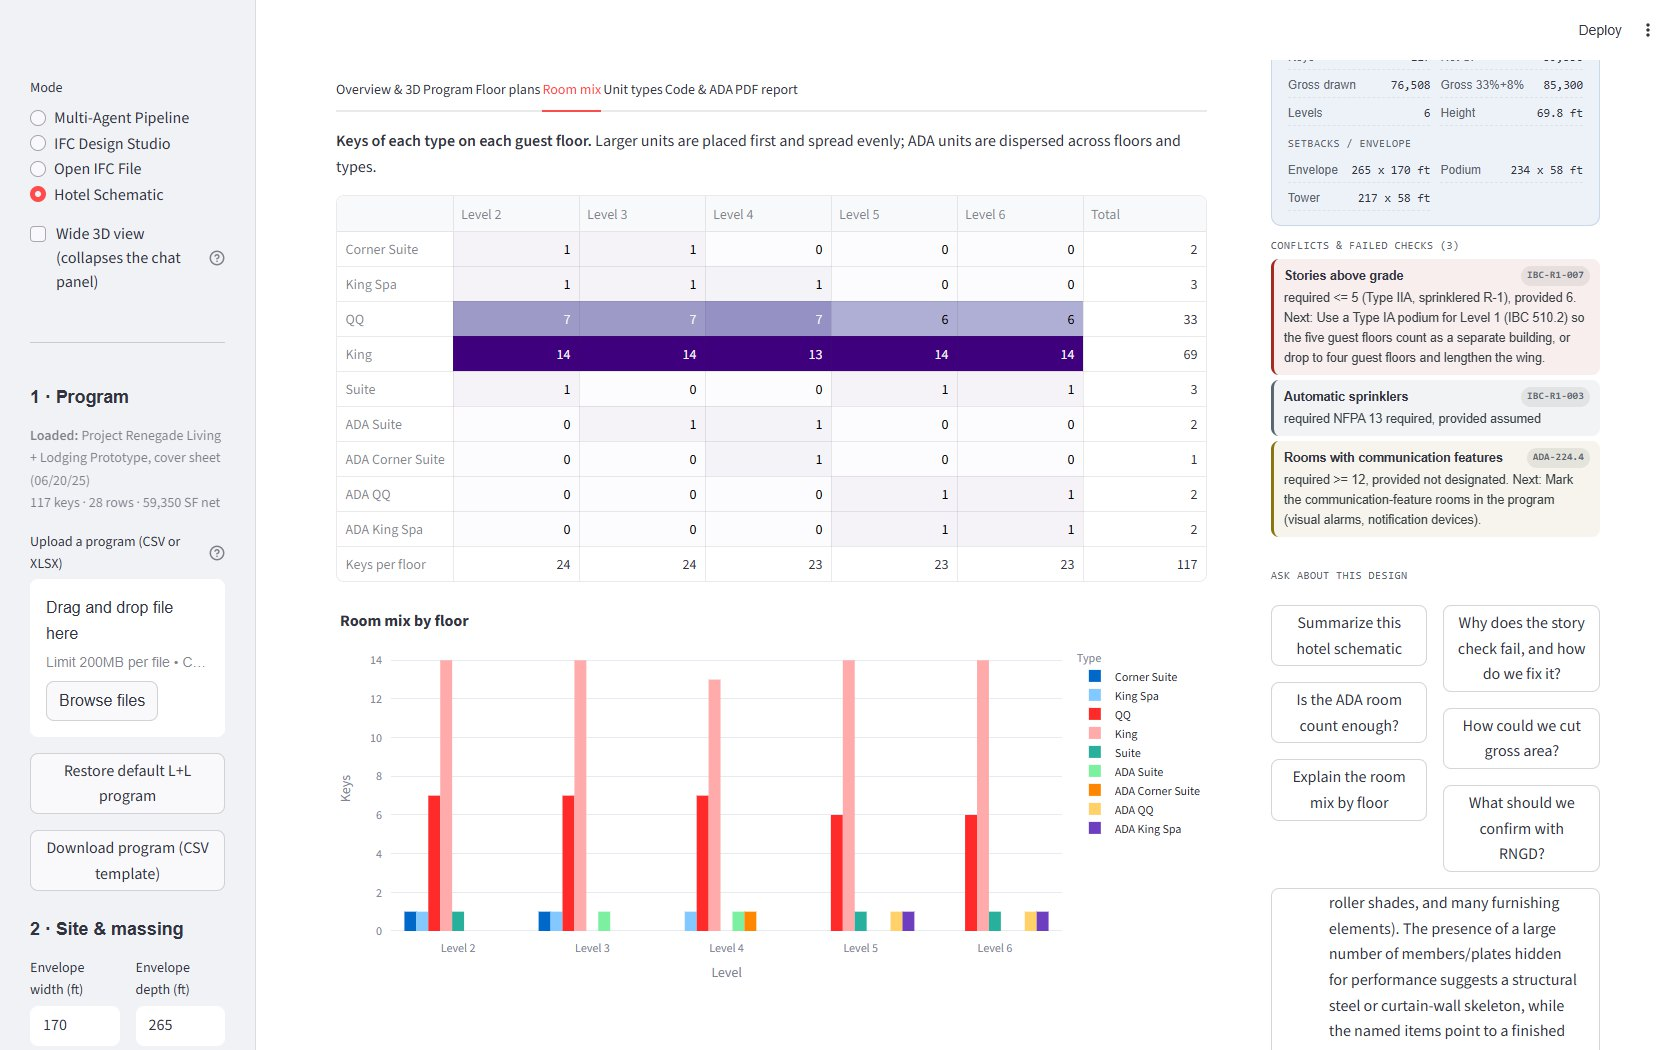
\includegraphics[width=0.92\linewidth,height=0.4\textheight,keepaspectratio]{figures/snap_26_hotel_room}\caption*{\textbf{Screen 26.} Keys of each room type on each guest floor.}\end{figure}
\begin{figure}[H]\centering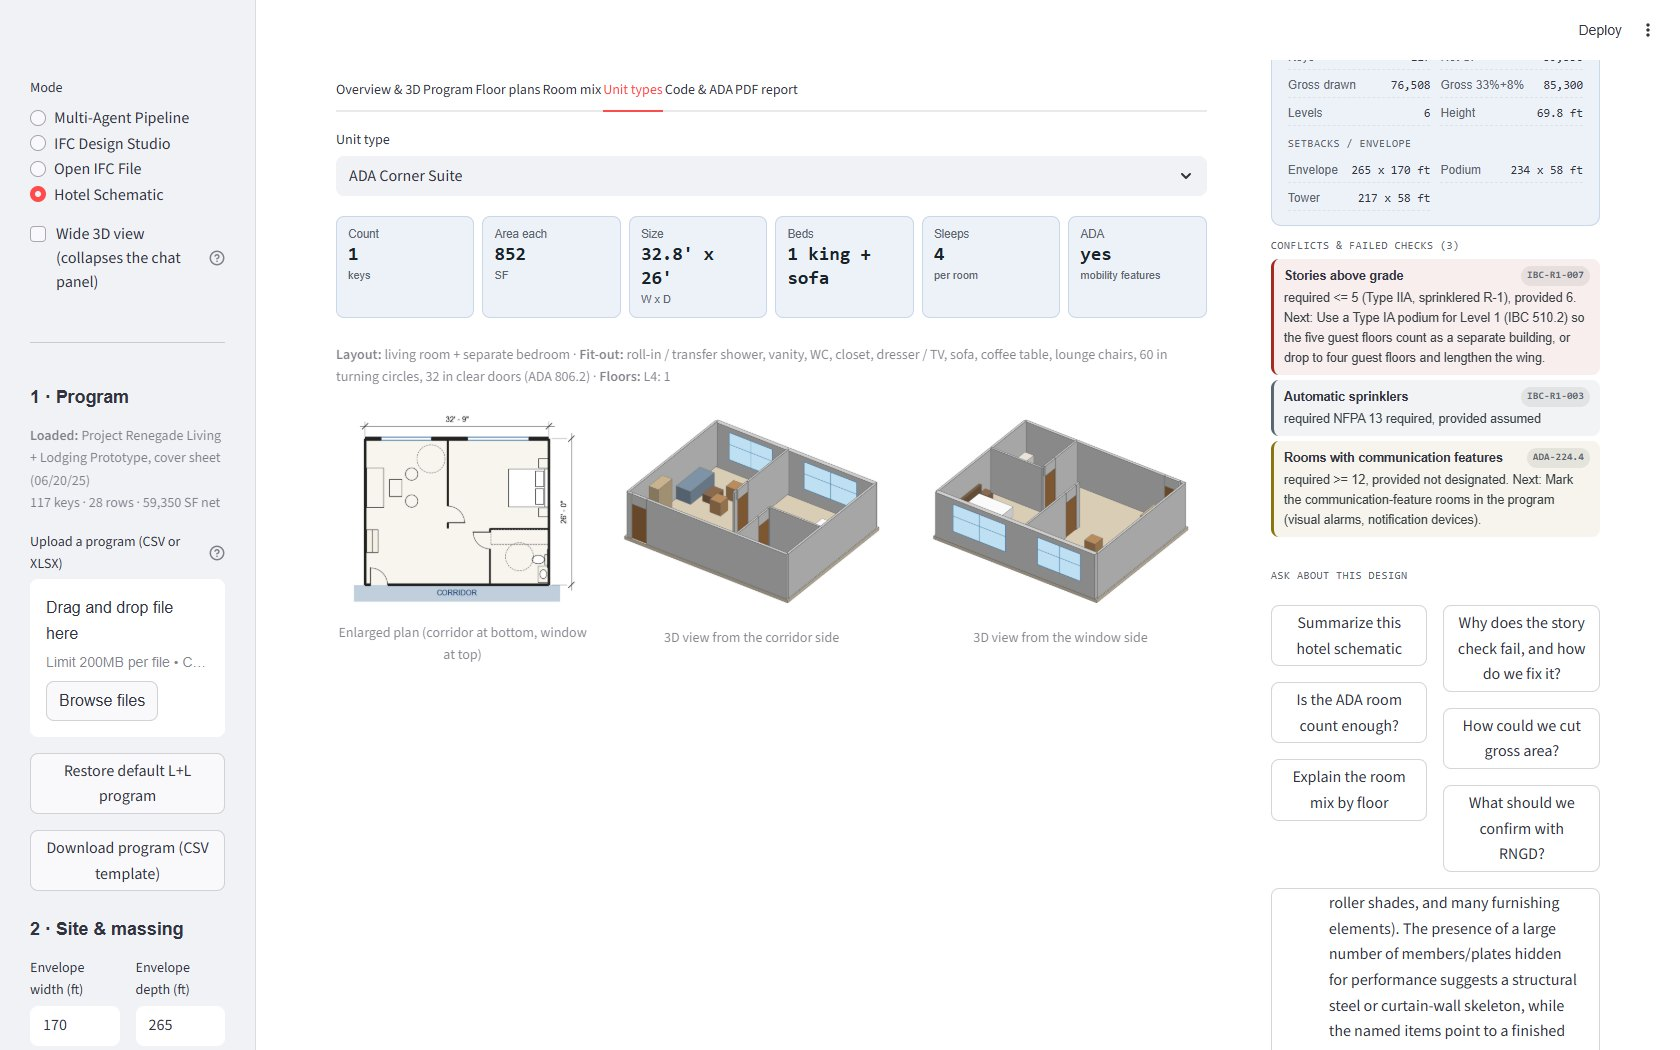
\includegraphics[width=0.92\linewidth,height=0.4\textheight,keepaspectratio]{figures/snap_27_hotel_unit}\caption*{\textbf{Screen 27.} Unit type detail: enlarged plan and two 3D interior views.}\end{figure}
\begin{figure}[H]\centering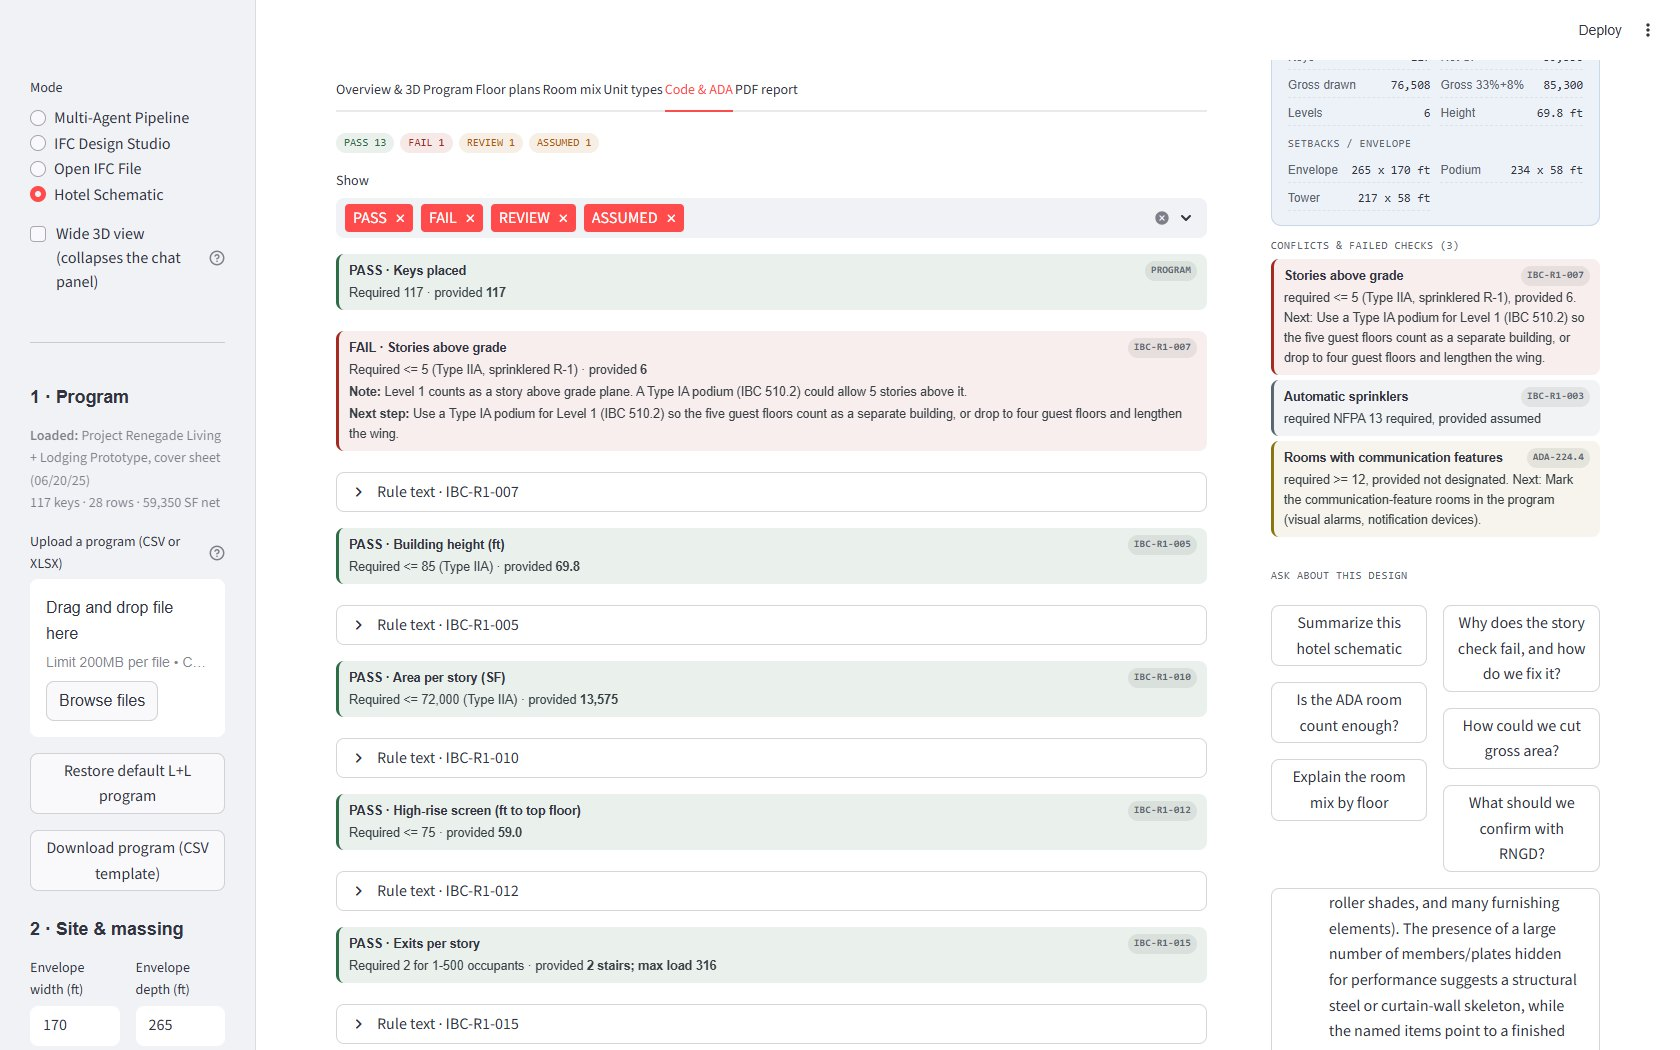
\includegraphics[width=0.92\linewidth,height=0.4\textheight,keepaspectratio]{figures/snap_28_hotel_code}\caption*{\textbf{Screen 28.} Code screen against RNGD's IBC rule set and the 2010 ADA guest-room tables, with rule text.}\end{figure}
\begin{figure}[H]\centering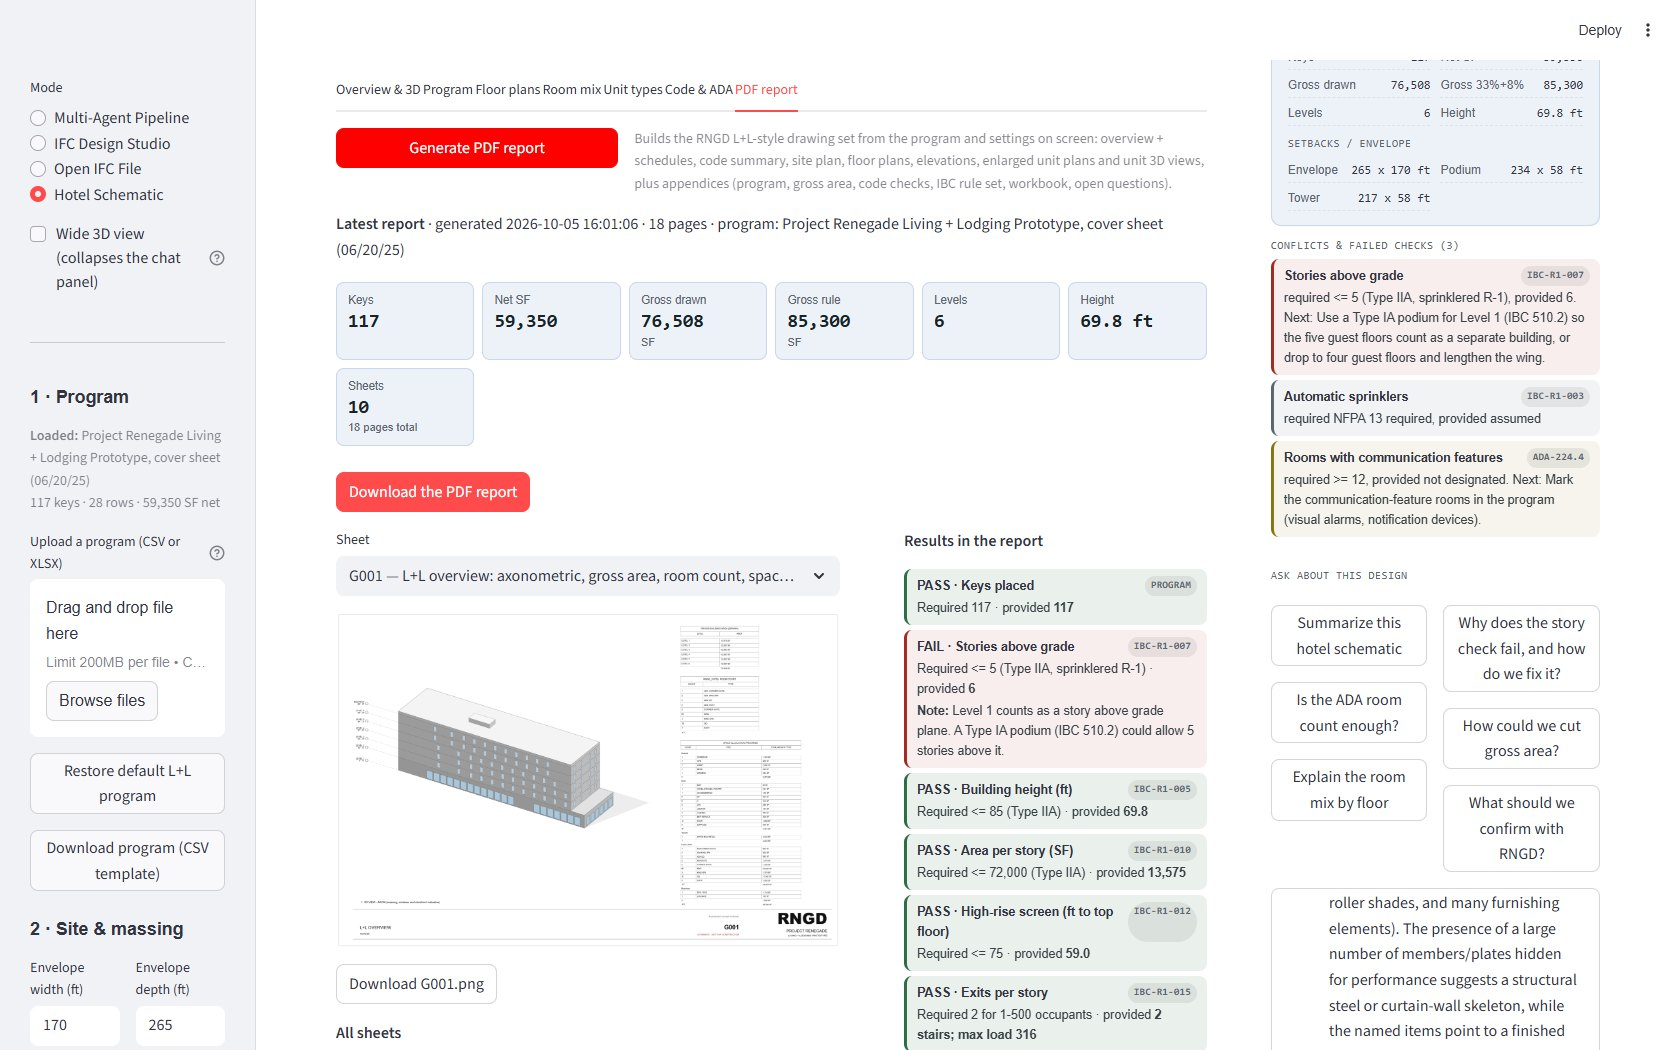
\includegraphics[width=0.92\linewidth,height=0.4\textheight,keepaspectratio]{figures/snap_29_hotel_report_results}\caption*{\textbf{Screen 29.} PDF report tab after generating: summary numbers and the results that went into the report.}\end{figure}
\begin{figure}[H]\centering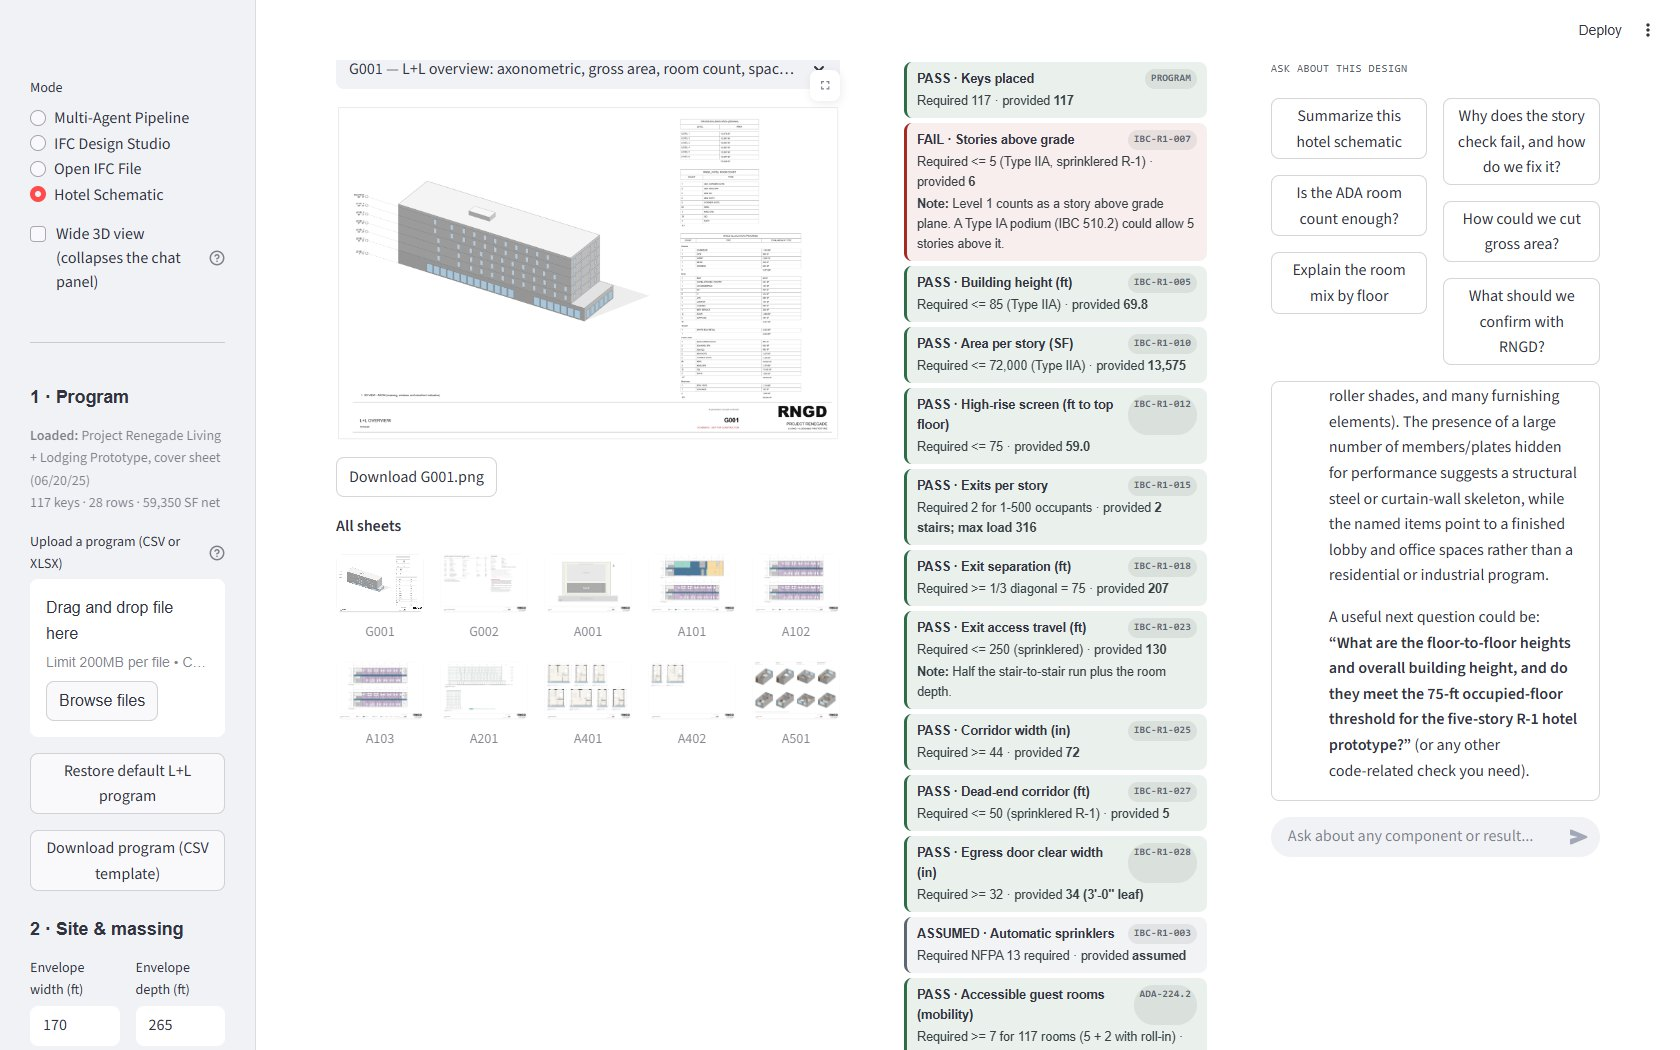
\includegraphics[width=0.92\linewidth,height=0.4\textheight,keepaspectratio]{figures/snap_30_hotel_report_sheets}\caption*{\textbf{Screen 30.} Sheet gallery of the generated drawing set.}\end{figure}
\subsection*{Assistant}
\begin{figure}[H]\centering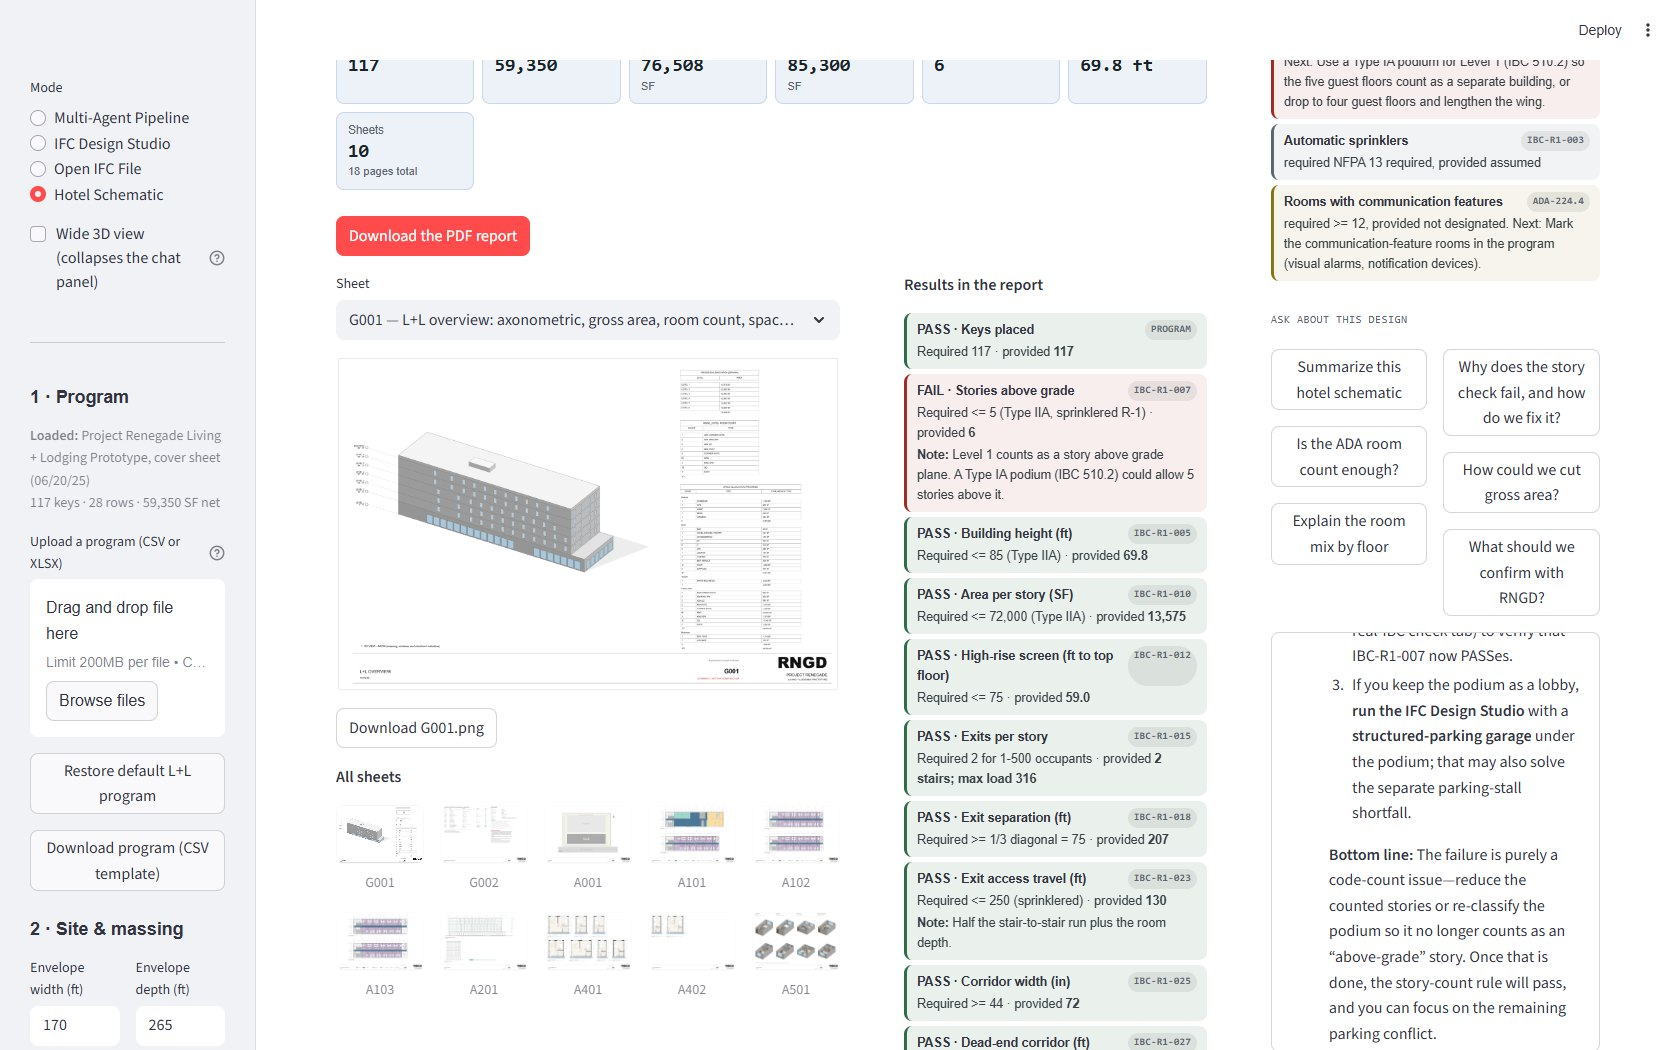
\includegraphics[width=0.92\linewidth,height=0.4\textheight,keepaspectratio]{figures/snap_31_assistant_answer}\caption*{\textbf{Screen 31.} The assistant answering a one-click question about the hotel design, using the live design state.}\end{figure}
